\documentclass[10pt,]{article}
\usepackage{lmodern}
\usepackage{amssymb,amsmath}
\usepackage{ifxetex,ifluatex}
\usepackage{fixltx2e} % provides \textsubscript
\ifnum 0\ifxetex 1\fi\ifluatex 1\fi=0 % if pdftex
  \usepackage[T1]{fontenc}
  \usepackage[utf8]{inputenc}
\else % if luatex or xelatex
  \ifxetex
    \usepackage{mathspec}
  \else
    \usepackage{fontspec}
  \fi
  \defaultfontfeatures{Ligatures=TeX,Scale=MatchLowercase}
\fi
% use upquote if available, for straight quotes in verbatim environments
\IfFileExists{upquote.sty}{\usepackage{upquote}}{}
% use microtype if available
\IfFileExists{microtype.sty}{%
\usepackage{microtype}
\UseMicrotypeSet[protrusion]{basicmath} % disable protrusion for tt fonts
}{}
\usepackage[margin=1in]{geometry}
\usepackage{hyperref}
\hypersetup{unicode=true,
            pdftitle={Projektaufgaben Block 2},
            pdfauthor={Carlo Michaelis, 573479; David Hinrichs, 572347; Lukas Ruff, 572521},
            pdfborder={0 0 0},
            breaklinks=true}
\urlstyle{same}  % don't use monospace font for urls
\usepackage{color}
\usepackage{fancyvrb}
\newcommand{\VerbBar}{|}
\newcommand{\VERB}{\Verb[commandchars=\\\{\}]}
\DefineVerbatimEnvironment{Highlighting}{Verbatim}{commandchars=\\\{\}}
% Add ',fontsize=\small' for more characters per line
\usepackage{framed}
\definecolor{shadecolor}{RGB}{248,248,248}
\newenvironment{Shaded}{\begin{snugshade}}{\end{snugshade}}
\newcommand{\KeywordTok}[1]{\textcolor[rgb]{0.13,0.29,0.53}{\textbf{{#1}}}}
\newcommand{\DataTypeTok}[1]{\textcolor[rgb]{0.13,0.29,0.53}{{#1}}}
\newcommand{\DecValTok}[1]{\textcolor[rgb]{0.00,0.00,0.81}{{#1}}}
\newcommand{\BaseNTok}[1]{\textcolor[rgb]{0.00,0.00,0.81}{{#1}}}
\newcommand{\FloatTok}[1]{\textcolor[rgb]{0.00,0.00,0.81}{{#1}}}
\newcommand{\ConstantTok}[1]{\textcolor[rgb]{0.00,0.00,0.00}{{#1}}}
\newcommand{\CharTok}[1]{\textcolor[rgb]{0.31,0.60,0.02}{{#1}}}
\newcommand{\SpecialCharTok}[1]{\textcolor[rgb]{0.00,0.00,0.00}{{#1}}}
\newcommand{\StringTok}[1]{\textcolor[rgb]{0.31,0.60,0.02}{{#1}}}
\newcommand{\VerbatimStringTok}[1]{\textcolor[rgb]{0.31,0.60,0.02}{{#1}}}
\newcommand{\SpecialStringTok}[1]{\textcolor[rgb]{0.31,0.60,0.02}{{#1}}}
\newcommand{\ImportTok}[1]{{#1}}
\newcommand{\CommentTok}[1]{\textcolor[rgb]{0.56,0.35,0.01}{\textit{{#1}}}}
\newcommand{\DocumentationTok}[1]{\textcolor[rgb]{0.56,0.35,0.01}{\textbf{\textit{{#1}}}}}
\newcommand{\AnnotationTok}[1]{\textcolor[rgb]{0.56,0.35,0.01}{\textbf{\textit{{#1}}}}}
\newcommand{\CommentVarTok}[1]{\textcolor[rgb]{0.56,0.35,0.01}{\textbf{\textit{{#1}}}}}
\newcommand{\OtherTok}[1]{\textcolor[rgb]{0.56,0.35,0.01}{{#1}}}
\newcommand{\FunctionTok}[1]{\textcolor[rgb]{0.00,0.00,0.00}{{#1}}}
\newcommand{\VariableTok}[1]{\textcolor[rgb]{0.00,0.00,0.00}{{#1}}}
\newcommand{\ControlFlowTok}[1]{\textcolor[rgb]{0.13,0.29,0.53}{\textbf{{#1}}}}
\newcommand{\OperatorTok}[1]{\textcolor[rgb]{0.81,0.36,0.00}{\textbf{{#1}}}}
\newcommand{\BuiltInTok}[1]{{#1}}
\newcommand{\ExtensionTok}[1]{{#1}}
\newcommand{\PreprocessorTok}[1]{\textcolor[rgb]{0.56,0.35,0.01}{\textit{{#1}}}}
\newcommand{\AttributeTok}[1]{\textcolor[rgb]{0.77,0.63,0.00}{{#1}}}
\newcommand{\RegionMarkerTok}[1]{{#1}}
\newcommand{\InformationTok}[1]{\textcolor[rgb]{0.56,0.35,0.01}{\textbf{\textit{{#1}}}}}
\newcommand{\WarningTok}[1]{\textcolor[rgb]{0.56,0.35,0.01}{\textbf{\textit{{#1}}}}}
\newcommand{\AlertTok}[1]{\textcolor[rgb]{0.94,0.16,0.16}{{#1}}}
\newcommand{\ErrorTok}[1]{\textcolor[rgb]{0.64,0.00,0.00}{\textbf{{#1}}}}
\newcommand{\NormalTok}[1]{{#1}}
\usepackage{longtable,booktabs}
\usepackage{graphicx,grffile}
\makeatletter
\def\maxwidth{\ifdim\Gin@nat@width>\linewidth\linewidth\else\Gin@nat@width\fi}
\def\maxheight{\ifdim\Gin@nat@height>\textheight\textheight\else\Gin@nat@height\fi}
\makeatother
% Scale images if necessary, so that they will not overflow the page
% margins by default, and it is still possible to overwrite the defaults
% using explicit options in \includegraphics[width, height, ...]{}
\setkeys{Gin}{width=\maxwidth,height=\maxheight,keepaspectratio}
\IfFileExists{parskip.sty}{%
\usepackage{parskip}
}{% else
\setlength{\parindent}{0pt}
\setlength{\parskip}{6pt plus 2pt minus 1pt}
}
\setlength{\emergencystretch}{3em}  % prevent overfull lines
\providecommand{\tightlist}{%
  \setlength{\itemsep}{0pt}\setlength{\parskip}{0pt}}
\setcounter{secnumdepth}{5}
% Redefines (sub)paragraphs to behave more like sections
\ifx\paragraph\undefined\else
\let\oldparagraph\paragraph
\renewcommand{\paragraph}[1]{\oldparagraph{#1}\mbox{}}
\fi
\ifx\subparagraph\undefined\else
\let\oldsubparagraph\subparagraph
\renewcommand{\subparagraph}[1]{\oldsubparagraph{#1}\mbox{}}
\fi

%%% Use protect on footnotes to avoid problems with footnotes in titles
\let\rmarkdownfootnote\footnote%
\def\footnote{\protect\rmarkdownfootnote}

%%% Change title format to be more compact
\usepackage{titling}

% Create subtitle command for use in maketitle
\newcommand{\subtitle}[1]{
  \posttitle{
    \begin{center}\large#1\end{center}
    }
}

\setlength{\droptitle}{-2em}
  \title{Projektaufgaben Block 2}
  \pretitle{\vspace{\droptitle}\centering\huge}
  \posttitle{\par}
  \author{Carlo Michaelis, 573479; David Hinrichs, 572347; Lukas Ruff, 572521}
  \preauthor{\centering\large\emph}
  \postauthor{\par}
  \predate{\centering\large\emph}
  \postdate{\par}
  \date{06 Dezember 2016}

\usepackage{amsthm}
\usepackage{amssymb}
\usepackage{amsmath}
\DeclareMathOperator*{\argmin}{argmin}
\usepackage{MnSymbol}
\usepackage{bbm}
\usepackage{subfig}
\usepackage{theoremref}
\newtheorem{satz}{Satz}

\begin{document}
\maketitle

\section{Nichtparametrisches Testen}\label{nichtparametrisches-testen}

\subsection{Zwillingsstudie}\label{zwillingsstudie}

Um zu testen, ob der Kindergartenbesuch einen signifikanten Einfluss auf
die sozialen Fähigkeiten eines Kindes hat, führen wir einen zweiseitigen
und einen einseitigen \(t\)-Test und einen zweiseitigen bzw. einseitigen
Wilcoxon-Vorzeichen-Test durch; jeweils zum Signifikanzniveau
\(\alpha = 0.05\).

\begin{Shaded}
\begin{Highlighting}[]
\CommentTok{# Enter data}
\NormalTok{x <-}\StringTok{ }\KeywordTok{c}\NormalTok{(}\DecValTok{82}\NormalTok{,}\DecValTok{69}\NormalTok{,}\DecValTok{73}\NormalTok{,}\DecValTok{43}\NormalTok{,}\DecValTok{58}\NormalTok{,}\DecValTok{56}\NormalTok{,}\DecValTok{76}\NormalTok{,}\DecValTok{65}\NormalTok{)}
\NormalTok{y <-}\StringTok{ }\KeywordTok{c}\NormalTok{(}\DecValTok{63}\NormalTok{,}\DecValTok{42}\NormalTok{,}\DecValTok{74}\NormalTok{,}\DecValTok{37}\NormalTok{,}\DecValTok{51}\NormalTok{,}\DecValTok{43}\NormalTok{,}\DecValTok{80}\NormalTok{,}\DecValTok{62}\NormalTok{)}
\NormalTok{testType <-}\StringTok{ }\KeywordTok{c}\NormalTok{(}\StringTok{'two-sided'}\NormalTok{, }\StringTok{'one-sided'}\NormalTok{)}
\NormalTok{pValueT <-}\StringTok{ }\KeywordTok{c}\NormalTok{(}\DecValTok{0}\NormalTok{,}\DecValTok{0}\NormalTok{); pValueWilcox <-}\StringTok{ }\KeywordTok{c}\NormalTok{(}\DecValTok{0}\NormalTok{,}\DecValTok{0}\NormalTok{)}

\CommentTok{# t-test}
\NormalTok{pValueT[}\DecValTok{1}\NormalTok{] <-}\StringTok{ }\KeywordTok{t.test}\NormalTok{(x, y, }\DataTypeTok{alternative =} \StringTok{"two.sided"}\NormalTok{, }\DataTypeTok{mu =} \DecValTok{0}\NormalTok{,}
                     \DataTypeTok{conf.level =} \FloatTok{0.95}\NormalTok{, }\DataTypeTok{paired =} \OtherTok{TRUE}\NormalTok{)$p.value}
\NormalTok{pValueT[}\DecValTok{2}\NormalTok{] <-}\StringTok{ }\KeywordTok{t.test}\NormalTok{(x, y, }\DataTypeTok{alternative =} \StringTok{"greater"}\NormalTok{, }\DataTypeTok{mu =} \DecValTok{0}\NormalTok{,}
                     \DataTypeTok{conf.level =} \FloatTok{0.95}\NormalTok{, }\DataTypeTok{paired =} \OtherTok{TRUE}\NormalTok{)$p.value}

\CommentTok{# Wilcoxon signed rank test}
\NormalTok{pValueWilcox[}\DecValTok{1}\NormalTok{] <-}\StringTok{ }\KeywordTok{wilcox.test}\NormalTok{(x, y, }\DataTypeTok{alternative =} \StringTok{"two.sided"}\NormalTok{,}
                               \DataTypeTok{mu =} \DecValTok{0}\NormalTok{, }\DataTypeTok{conf.level =} \FloatTok{0.95}\NormalTok{, }
            \DataTypeTok{paired =} \OtherTok{TRUE}\NormalTok{, }\DataTypeTok{conf.int =} \OtherTok{TRUE}\NormalTok{)$p.value}
\NormalTok{pValueWilcox[}\DecValTok{2}\NormalTok{] <-}\StringTok{ }\KeywordTok{wilcox.test}\NormalTok{(x, y, }\DataTypeTok{alternative =} \StringTok{"greater"}\NormalTok{,}
                               \DataTypeTok{mu =} \DecValTok{0}\NormalTok{, }\DataTypeTok{conf.level =} \FloatTok{0.95}\NormalTok{, }
            \DataTypeTok{paired =} \OtherTok{TRUE}\NormalTok{, }\DataTypeTok{conf.int =} \OtherTok{TRUE}\NormalTok{)$p.value}


\NormalTok{knitr::}\KeywordTok{kable}\NormalTok{(}\KeywordTok{data.frame}\NormalTok{(testType, pValueT, pValueWilcox), }\DataTypeTok{caption =} \StringTok{'p-Werte'}\NormalTok{)}
\end{Highlighting}
\end{Shaded}

\begin{longtable}[]{@{}lrr@{}}
\caption{p-Werte}\tabularnewline
\toprule
testType & pValueT & pValueWilcox\tabularnewline
\midrule
\endfirsthead
\toprule
testType & pValueT & pValueWilcox\tabularnewline
\midrule
\endhead
two-sided & 0.0489476 & 0.0546875\tabularnewline
one-sided & 0.0244738 & 0.0273438\tabularnewline
\bottomrule
\end{longtable}

\textbf{Zweiseitige Tests}

Wir können sehen, dass der \(t\)-Test die Nullhypothese ablehnt
(\(p = 0.04895 < \alpha\)) und somit einen signifikanten Einfluss des
Kindergartenbesuchs auf die sozialen Fähigkeiten feststellt. Der
Wilcoxon-Vorzeichen-Test hingegen (\(p = 0.0546875 < \alpha\)) lehnt die
Nullhypothese hingegen nicht zum gegebenen Signifikanzniveau ab und
spricht somit gegen einen entsprechenden Einfluss.

\textbf{Einseitige Tests}

Nehmen wir von vorne herein an, dass die sozialen Fähigkeiten
signifikant höher sind, wenn die Kinder den Kindergarten besuchen, dann
formulieren wir einen einseitigen Test. Unter dieser Annahme sprechen
beide Tests gegen die Nullhypothese.

Der Grund liegt darin, dass hier die \(p\)-Werte nur eine Ablehnregion
in die Richtung ``größer'' abdecken müssen und aufgrund der Symmetrie
der Tests deshalb nur halb so groß sind wie bei den zweiseitigen Tests.
Beide Tests indizieren nun einen signifikanten Anstieg der sozialen
Fähigkeiten durch den Kindergartenbesuch.

\textbf{Testannahmen}

Schließlich lohnt es, einen Blick auf die Testannahmen zu richten.
Während der Wilcoxon-Test lediglich eine symmetrische Verteilung
voraussetzt, nimmt der t-Test konkret die Normalverteilung,
\(X_i - Y_i \sim N(0,\sigma^2)\), der Daten an. Da diese stärkere
Annahme ihm auch zu seiner größeren Power verhilft, sollte man ihre
Validität überprüfen, hier geschieht dies mit Hilfe eines QQ-Plot:

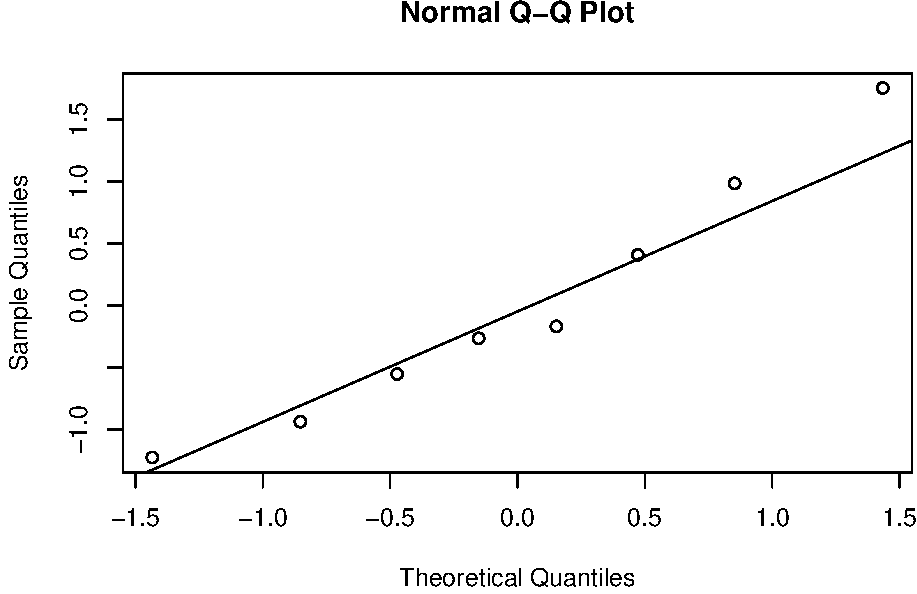
\includegraphics{project2_files/figure-latex/Normalverteilungsannahme-1.pdf}

Wie besonders am rechten Tail zu erkennen, kann die
Normalverteilungsannahme durchaus in Frage gestellt werden.

Doch auch die Annahme symmetrischer Daten ist angesichts der ``Schiefe''
(2.25) der Daten anzuzweifeln, aber sie ist deutlich schwächer als die
zusätzliche Annahme einer (bis auf Paramter) exakten Verteilung.

Das Hauptproblem dieser Stichprobe ist jedoch ihre geringe Größe von N =
8, jedwede Art von Statistik besitzt in diesem Fall nur sehr geringe
Aussagekraft.

\subsection{\texorpdfstring{\(t\)-Test
vs.~Wilcoxon-Vorzeichen-Test}{t-Test vs.~Wilcoxon-Vorzeichen-Test}}\label{t-test-vs.wilcoxon-vorzeichen-test}

Als nächstes schätzen wir die Power beider Tests in verschiedenen
Settings ab. Dafür wird zunächst der wahre Wert
\(\theta \in [0, 0.5, 1]\) mit Fehlern verrauscht, die der Normal-,
Cauchy-, und Gleichverteilung folgen. Die Funktion, welche die
entsprechend verteilten Daten erzeugt, wird mittels \texttt{fnError}
übergeben. Die Erzeugung der Daten wird mehrfach durchgeführt und mit
den beiden Tests getestet (Monte-Carlo-Simulation). Die Nullhypothese
lautet dabei in jedem Fall, dass \(\theta = 0\). Nach der Durchführung
der Tests werden jeweils die \(p\)-Werte bestimmt und gemittelt, und
aufgrund der Form der Tests
\(\phi =1(p(X_1,...,X_n) < \alpha) = 1(p_i<\alpha)\) mit dem p-Wert des
\(p\), ergibt sich die mittlere Power für \(m= nSim = 10.000\)
Mote-Carlo-Simulationen als
\(\beta_m = \frac{1}{m}\sum_{i=1}^{m}{\phi_i} = \frac{1}{m}\sum_{i=1}^{m}{1(p_i<\alpha)}\).

\begin{Shaded}
\begin{Highlighting}[]
\NormalTok{fnTestPowerMC <-}\StringTok{ }\NormalTok{function(fnError, }\DataTypeTok{n =} \DecValTok{30}\NormalTok{, }\DataTypeTok{alpha =} \FloatTok{0.05}\NormalTok{, }\DataTypeTok{nSim =} \DecValTok{10}\NormalTok{^}\DecValTok{4}\NormalTok{, ...) \{}
  \CommentTok{# This function estimates the probability of rejecting the null hypothesis of a}
  \CommentTok{# t-test and a Wilcoxon signed rank test using Monte Carlo simulations of iid}
  \CommentTok{# random variables X_i = \textbackslash{}theta + \textbackslash{}epsilon_i.}
  \CommentTok{# }
  \CommentTok{# Args:}
  \CommentTok{#   fnError:  Function which generates random samples from a symmetric error }
  \CommentTok{#             distribution \textbackslash{}epsilon}
  \CommentTok{#   n:        Number of random samples used in tests}
  \CommentTok{#   alpha:    Significance level used in tests}
  \CommentTok{#   nSim:     Number of MC simulations of size n}
  \CommentTok{#   ...:      Further arguments to be passed to fnError}
  \CommentTok{#   }
  \CommentTok{# Returns:}
  \CommentTok{#   A list containing the following elements:}
  \CommentTok{#     $TProb:       MC estimation of rejection probability for the t-test}
  \CommentTok{#     $WilcoxProb:  MC estimation of rejection probability for the Wilcoxon}
  \CommentTok{#                   signed rank test}
  
  \CommentTok{# Perform MC simulation}
  \NormalTok{matX <-}\StringTok{ }\KeywordTok{matrix}\NormalTok{(}\KeywordTok{fnError}\NormalTok{(n*nSim, ...), }\DataTypeTok{ncol =} \NormalTok{n)}
  
  \CommentTok{# Define sub-functions which only return p-values from the two tests}
  \NormalTok{fnPvalT <-}\StringTok{ }\NormalTok{function(x) \{}
    \KeywordTok{return}\NormalTok{(}\KeywordTok{t.test}\NormalTok{(x)$p.value)}
  \NormalTok{\}}
  \NormalTok{fnPvalWilcox <-}\StringTok{ }\NormalTok{function(x) \{}
    \KeywordTok{return}\NormalTok{(}\KeywordTok{wilcox.test}\NormalTok{(x)$p.value)}
  \NormalTok{\}}
  
  \CommentTok{# Perform nSim number of tests with sample size n for each of the two tests}
  \NormalTok{vecPvalT <-}\StringTok{ }\KeywordTok{apply}\NormalTok{(matX, }\DecValTok{1}\NormalTok{, fnPvalT)}
  \NormalTok{vecPvalWilcox <-}\StringTok{ }\KeywordTok{apply}\NormalTok{(matX, }\DecValTok{1}\NormalTok{, fnPvalWilcox)}
  
  \CommentTok{# Compute and return estimations of rejection probabilities}
  \NormalTok{result <-}\StringTok{ }\KeywordTok{list}\NormalTok{()}
  \NormalTok{result$TProb <-}\StringTok{ }\KeywordTok{mean}\NormalTok{(vecPvalT <}\StringTok{ }\NormalTok{alpha)}
  \NormalTok{result$WilcoxProb <-}\StringTok{ }\KeywordTok{mean}\NormalTok{(vecPvalWilcox <}\StringTok{ }\NormalTok{alpha)}
  \KeywordTok{return}\NormalTok{(result)}
\NormalTok{\}}
\end{Highlighting}
\end{Shaded}

\begin{Shaded}
\begin{Highlighting}[]
\CommentTok{# Set seed}
\KeywordTok{set.seed}\NormalTok{(}\DecValTok{432}\NormalTok{)}

\CommentTok{# Normal errors}
\NormalTok{normalMean =}\StringTok{ }\KeywordTok{c}\NormalTok{(}\DecValTok{0}\NormalTok{, }\FloatTok{0.5}\NormalTok{, }\DecValTok{1}\NormalTok{)}
\NormalTok{normalSD =}\StringTok{ }\KeywordTok{c}\NormalTok{(}\DecValTok{1}\NormalTok{, }\DecValTok{1}\NormalTok{, }\DecValTok{1}\NormalTok{)}
\NormalTok{normalPowerT <-}\StringTok{ }\KeywordTok{list}\NormalTok{()}
\NormalTok{normalPowerW <-}\StringTok{ }\KeywordTok{list}\NormalTok{()}

\NormalTok{for (i in }\DecValTok{1}\NormalTok{:}\DecValTok{3}\NormalTok{) \{}
  \NormalTok{res <-}\StringTok{ }\KeywordTok{fnTestPowerMC}\NormalTok{(}\DataTypeTok{fnError =} \NormalTok{rnorm, }\DataTypeTok{nSim =} \DecValTok{10}\NormalTok{^}\DecValTok{4}\NormalTok{,}
                       \DataTypeTok{mean =} \NormalTok{normalMean[i], }\DataTypeTok{sd=}\NormalTok{normalSD[i])}
  \NormalTok{normalPowerT[i] <-}\StringTok{ }\NormalTok{res[}\DecValTok{1}\NormalTok{]}
  \NormalTok{normalPowerW[i] <-}\StringTok{ }\NormalTok{res[}\DecValTok{2}\NormalTok{]}
\NormalTok{\}}

\CommentTok{# Uniform errors}
\NormalTok{uniMin <-}\StringTok{ }\KeywordTok{c}\NormalTok{(-}\DecValTok{1}\NormalTok{, -}\FloatTok{0.5}\NormalTok{, }\DecValTok{0}\NormalTok{)}
\NormalTok{uniMax <-}\StringTok{ }\KeywordTok{c}\NormalTok{(}\DecValTok{1}\NormalTok{, }\FloatTok{1.5}\NormalTok{, }\DecValTok{2}\NormalTok{)}
\NormalTok{uniPowerT <-}\StringTok{ }\KeywordTok{list}\NormalTok{()}
\NormalTok{uniPowerW <-}\StringTok{ }\KeywordTok{list}\NormalTok{()}

\NormalTok{for (i in }\DecValTok{1}\NormalTok{:}\DecValTok{3}\NormalTok{) \{}
  \NormalTok{res <-}\StringTok{ }\KeywordTok{fnTestPowerMC}\NormalTok{(}\DataTypeTok{fnError =} \NormalTok{runif, }\DataTypeTok{nSim =} \DecValTok{10}\NormalTok{^}\DecValTok{4}\NormalTok{,}
                       \DataTypeTok{min =} \NormalTok{uniMin[i], }\DataTypeTok{max =} \NormalTok{uniMax[i])}
  \NormalTok{uniPowerT[i] <-}\StringTok{ }\NormalTok{res[}\DecValTok{1}\NormalTok{]}
  \NormalTok{uniPowerW[i] <-}\StringTok{ }\NormalTok{res[}\DecValTok{2}\NormalTok{]}
\NormalTok{\}}

\CommentTok{# Cauchy errors (t-distribution with df = 1)}
\NormalTok{cauchyPowerT <-}\StringTok{ }\KeywordTok{list}\NormalTok{()}
\NormalTok{cauchyPowerW <-}\StringTok{ }\KeywordTok{list}\NormalTok{()}
\NormalTok{cauchyLoc =}\StringTok{ }\KeywordTok{c}\NormalTok{(}\DecValTok{0}\NormalTok{, }\FloatTok{0.5}\NormalTok{, }\DecValTok{1}\NormalTok{)}
\NormalTok{cauchyScale =}\StringTok{ }\KeywordTok{c}\NormalTok{(}\DecValTok{1}\NormalTok{,}\DecValTok{1}\NormalTok{,}\DecValTok{1}\NormalTok{)}
\NormalTok{for (i in }\DecValTok{1}\NormalTok{:}\DecValTok{3}\NormalTok{) \{}
  \NormalTok{res <-}\StringTok{ }\KeywordTok{fnTestPowerMC}\NormalTok{(}\DataTypeTok{fnError =} \NormalTok{rcauchy, }\DataTypeTok{nSim =} \DecValTok{10}\NormalTok{^}\DecValTok{4}\NormalTok{,}
                       \DataTypeTok{location =} \NormalTok{cauchyLoc[i], }\DataTypeTok{scale=}\NormalTok{cauchyScale[i])}
  \NormalTok{cauchyPowerT[i] <-}\StringTok{ }\NormalTok{res[}\DecValTok{1}\NormalTok{]}
  \NormalTok{cauchyPowerW[i] <-}\StringTok{ }\NormalTok{res[}\DecValTok{2}\NormalTok{]}
\NormalTok{\}}
\end{Highlighting}
\end{Shaded}

\begin{longtable}[]{@{}rrrr@{}}
\caption{Normalverteilte Daten}\tabularnewline
\toprule
mean & sd & power T-test & power Wilcox-test\tabularnewline
\midrule
\endfirsthead
\toprule
mean & sd & power T-test & power Wilcox-test\tabularnewline
\midrule
\endhead
0.0 & 1 & 0.0492 & 0.0506\tabularnewline
0.5 & 1 & 0.7528 & 0.7387\tabularnewline
1.0 & 1 & 0.9992 & 0.9990\tabularnewline
\bottomrule
\end{longtable}

\begin{longtable}[]{@{}rrrr@{}}
\caption{Gleichverteilte Daten}\tabularnewline
\toprule
mean & +- interval & power T-test & power Wilcox-test\tabularnewline
\midrule
\endfirsthead
\toprule
mean & +- interval & power T-test & power Wilcox-test\tabularnewline
\midrule
\endhead
0.0 & 1 & 0.0500 & 0.0478\tabularnewline
0.5 & 1 & 0.9979 & 0.9876\tabularnewline
1.0 & 1 & 1.0000 & 1.0000\tabularnewline
\bottomrule
\end{longtable}

\begin{longtable}[]{@{}rrrr@{}}
\caption{Cauchyverteilte Daten}\tabularnewline
\toprule
location & scale & power T-test & power Wilcox-test\tabularnewline
\midrule
\endfirsthead
\toprule
location & scale & power T-test & power Wilcox-test\tabularnewline
\midrule
\endhead
0.0 & 1 & 0.0193 & 0.0508\tabularnewline
0.5 & 1 & 0.0735 & 0.2957\tabularnewline
1.0 & 1 & 0.2010 & 0.6996\tabularnewline
\bottomrule
\end{longtable}

\textbf{Normalverteilte Daten}

Wie bereits aus dem ersten Teil der Aufgabe zu erwarten, sind die
Unterschiede der \(p\)-Werte nicht sehr groß. Gleichzeitig nehmen die
\(p\)-Werte drastisch zu, wenn der Erwartungswert bei der Erzeugung der
Daten verschoben wird. Die starke Zunahme lässt sich vermutlich damit
erklären, dass die Varianz der Teststatistik auf Grund der
Stichprobengröße sehr klein wird.

\textbf{Gleichverteilte Daten}

Die \(p\)-Werte der gleichverteilten Daten für \(t\)-Test und
Wilcox-Test sind relativ ähnlich. Obwohl also keine Normalverteilung der
Zufallsvariable vorliegt, scheint der \(t\)-Test (der eigentlich auf
dieser Annahme basiert) noch eine relativ gute Leitsung zu haben,
zumindest verglichen mit dem Wilcox-Test. Dass die \(p\)-Werte mit
zunehmender Verschiebung stark zunehmen, hat vermutlich zwei Ursachen.
Neben der abnehmenden Varianz (wie oben), sind die Daten bei der
Gleichverteilung beschränkt. Bspw. ist bei \(\theta = 1\) und einer
Gleichverteilung im Bereich \([0,2]\) (letzter Fall) intuitiv sehr
deutlich zu erkennen, dass Werte mit Null nur sehr selten vorkommen.
Wenn gleichzeitig die Varianz der Teststatistik mit zunehmender
Stichprobengröße abnimmt (und im Fall \(\theta = 0,5\) wird deutlich,
dass sie sehr klein zu sein scheint), wird klar, warum wir diesem Fall
\(p = 1\) als Ergebnis erhalten.

\textbf{Cauchyverteilte Daten}

Die cauchyverteilten Daten führen zu starken Differenzen zwischen den
\(p\)-Werten der beiden Tests. Die Verletzung der
Normalverteilungs-Annahme hat hier offensichtlich deutlich größere
Auswirkungen, als bspw. im Fall der Gleichverteilung. Auf Grund der
massereichen Tails der Cauchyverteilung, kann die Varianz der
Teststatistik durch die Stichprobengröße nicht effektiv genug verringert
werden und es kommt auch im Bereich von \(\theta = 0,5\) und
\(\theta = 1\) noch zu vergleichsweise kleinen \(p\)-Werten.

\section{Dichteschätzung}\label{dichteschatzung}

In dieser Aufgabe ist es unser Ziel eine unbekannte Dichte \(f\) mittels
Sample \(X_1, \ldots, X_n \overset{iid}{\sim} \mathbb{P}_f\) zu
approximieren. Für die Schätzung untersuchen und verwenden wir eine
nichtparametrische Methode - den Kerndichteschätzer. Wir werden sehen,
dass die „Güte`` der Approximation von der Wahl des Kerns \(K\) sowie
von der Bandweitenwahl \(h\) abhängt und werden versuchen zu gegebenem
Kern \(K\) mittels Kreuzvalidierung eine „optimale`` Bandweite zu
wählen.

\subsection{Kerndichteschätzer}\label{kerndichteschatzer}

Für gegebene Daten \(X_1, \ldots, X_n\) können wir einen allgemeinen
Kerndichteschätzer \(\hat{f}_n\) für einen Kern \(K\) und Bandweite
\(h\) wie folgt für einen Vektor von Stellen \texttt{x} implementieren:

\begin{Shaded}
\begin{Highlighting}[]
\NormalTok{fnKernelDensityEst <-}\StringTok{ }\NormalTok{function(x, X, K, h) \{}
  \CommentTok{# This function computes the kernel density estimates for a given sample X and}
  \CommentTok{# kernel K with bandwidth h at points x.}
  \CommentTok{# }
  \CommentTok{# Args:}
  \CommentTok{#   x: Points for which the kernel density estimates are computed}
  \CommentTok{#   X: Data sample on which the kernel density estimation is fitted}
  \CommentTok{#   K: Kernel function to be used for smoothing}
  \CommentTok{#   h: Smoothing bandwidth}
  \CommentTok{#   }
  \CommentTok{# Returns:}
  \CommentTok{#   A vector of the kernel density estimates at points x}
  
  \CommentTok{# Compute kernel density estimation values using outer}
  \NormalTok{n <-}\StringTok{ }\KeywordTok{length}\NormalTok{(X)}
  \NormalTok{mKernels <-}\StringTok{ }\KeywordTok{K}\NormalTok{((}\DecValTok{1}\NormalTok{/h) *}\StringTok{ }\KeywordTok{outer}\NormalTok{(X, x, }\DataTypeTok{FUN =} \StringTok{"-"}\NormalTok{))}
  \KeywordTok{return}\NormalTok{((}\DecValTok{1}\NormalTok{/(n*h)) *}\StringTok{ }\KeywordTok{colSums}\NormalTok{(mKernels))}
\NormalTok{\}}
\end{Highlighting}
\end{Shaded}

Bevor wir die Methode für Zufallszahlen verschiedener Verteilungen
testen, implementieren wir noch drei Kerne (Rechtseckskern, Gaußkern,
Epanechnikov-Kern) und schreiben eine allgemeine Funktion zur Erstellung
von Plots (welche bereits für die spätere Anwendung der \(m\)-nächste
Nachbarn Methode angepasst wurde):

\begin{Shaded}
\begin{Highlighting}[]
\CommentTok{# Define different smoothing kernels}

\NormalTok{fnRectangularKernel <-}\StringTok{ }\NormalTok{function(x) \{}
  \KeywordTok{return}\NormalTok{(}\FloatTok{0.5} \NormalTok{*}\StringTok{ }\NormalTok{(}\KeywordTok{abs}\NormalTok{(x) <=}\StringTok{ }\DecValTok{1}\NormalTok{))}
\NormalTok{\}}

\NormalTok{fnGaussianKernel <-}\StringTok{ }\NormalTok{function(x) \{}
  \KeywordTok{return}\NormalTok{((}\DecValTok{1}\NormalTok{/}\KeywordTok{sqrt}\NormalTok{(}\DecValTok{2}\NormalTok{*pi)) *}\StringTok{ }\KeywordTok{exp}\NormalTok{((-}\FloatTok{0.5}\NormalTok{) *}\StringTok{ }\NormalTok{x^}\DecValTok{2}\NormalTok{))}
\NormalTok{\}}

\NormalTok{fnEpanechnikovKernel <-}\StringTok{ }\NormalTok{function(x) \{}
  \KeywordTok{return}\NormalTok{(}\FloatTok{0.75} \NormalTok{*}\StringTok{ }\NormalTok{(}\DecValTok{1} \NormalTok{-}\StringTok{ }\NormalTok{x^}\DecValTok{2}\NormalTok{) *}\StringTok{ }\NormalTok{(}\KeywordTok{abs}\NormalTok{(x) <=}\StringTok{ }\DecValTok{1}\NormalTok{))}
\NormalTok{\}}
\end{Highlighting}
\end{Shaded}

\begin{Shaded}
\begin{Highlighting}[]
\NormalTok{fnKernelPlot <-}\StringTok{ }\NormalTok{function(x, X, K, }\DataTypeTok{vh =} \OtherTok{NULL}\NormalTok{, }\DataTypeTok{vm =} \OtherTok{NULL}\NormalTok{,}
                         \DataTypeTok{fnEstimation =} \NormalTok{fnKernelDensityEst,}
                         \DataTypeTok{title =} \OtherTok{NULL}\NormalTok{, }\DataTypeTok{trueDensity =} \OtherTok{NULL}\NormalTok{, ...) \{}
  \CommentTok{# This function plots the kernel density estimates for different bandwidths.}
  \CommentTok{# If trueDensity is specified, the true density will be plotted as well.}
  \CommentTok{# }
  \CommentTok{# Args:}
  \CommentTok{#   x:            Points for which the kernel density estimates are computed}
  \CommentTok{#   X:            Data sample on which the kernel density estimation is fitted}
  \CommentTok{#   K:            Kernel function to be used for smoothing}
  \CommentTok{#   vh:           Vector of smoothing bandwidths}
  \CommentTok{#   vm:           Vector of nearest neighbor positions}
  \CommentTok{#   fnEstimation: Type of estimation used (kernel density or knn)}
  \CommentTok{#   title:        Main title of the plot}
  \CommentTok{#   trueDensity:  True density to be plotted (e.g. dnorm)}
  \CommentTok{#   ...:          Further arguments passed to or from other methods}
  \CommentTok{#   }
  \CommentTok{# Returns:}
  \CommentTok{#   -}
  
  \NormalTok{if(!}\KeywordTok{is.null}\NormalTok{(vh)) \{}
    \NormalTok{vPar <-}\StringTok{ }\NormalTok{vh}
    \NormalTok{strPar <-}\StringTok{ "h"}
  \NormalTok{\} else if(!}\KeywordTok{is.null}\NormalTok{(vm)) \{}
    \NormalTok{vPar <-}\StringTok{  }\NormalTok{vm}
    \NormalTok{strPar <-}\StringTok{ "m"}
  \NormalTok{\} else \{}
    \KeywordTok{stop}\NormalTok{(}\StringTok{"You need to set bandwiths vh OR neighbor ranks vm"}\NormalTok{)}
  \NormalTok{\}}
  
  \NormalTok{nPar <-}\StringTok{ }\KeywordTok{length}\NormalTok{(vPar)}
  
  \CommentTok{# Create color palette for number of hyperparameters}
  \NormalTok{cols <-}\StringTok{ }\KeywordTok{rainbow}\NormalTok{(nPar, }\DataTypeTok{alpha =} \DecValTok{1}\NormalTok{)}
  
  \CommentTok{# Initialize plot with first kernel density}
  \KeywordTok{plot}\NormalTok{(x, }\KeywordTok{fnEstimation}\NormalTok{(x, X, K, vPar[}\DecValTok{1}\NormalTok{]), }\DataTypeTok{type =} \StringTok{"l"}\NormalTok{, }\DataTypeTok{col =} \NormalTok{cols[}\DecValTok{1}\NormalTok{], }
       \DataTypeTok{main =} \NormalTok{title, }\DataTypeTok{xlab =} \StringTok{"x"}\NormalTok{, }\DataTypeTok{ylab =} \StringTok{"Density"}\NormalTok{, ...)}
  
  \CommentTok{# Add kernel density for each additional bandwidth}
  \NormalTok{if (nPar >}\StringTok{ }\DecValTok{1}\NormalTok{) \{}
    \NormalTok{for (i in }\DecValTok{2}\NormalTok{:nPar) \{}
      \KeywordTok{lines}\NormalTok{(x, }\KeywordTok{fnEstimation}\NormalTok{(x, X, K, vPar[i]), }\DataTypeTok{col =} \NormalTok{cols[i])}
    \NormalTok{\}}
  \NormalTok{\}}
  
  \CommentTok{# Create legend}
  \NormalTok{legend <-}\StringTok{ }\KeywordTok{sapply}\NormalTok{(vPar, function(par) \{}\KeywordTok{paste}\NormalTok{(strPar, }\StringTok{" = "}\NormalTok{, }\KeywordTok{round}\NormalTok{(par, }\DecValTok{4}\NormalTok{))\})}
  
  \CommentTok{# Plot true density if specified}
  \NormalTok{if (!}\KeywordTok{is.null}\NormalTok{(trueDensity)) \{}
    \KeywordTok{lines}\NormalTok{(x, }\KeywordTok{trueDensity}\NormalTok{(x), }\DataTypeTok{col =} \StringTok{"black"}\NormalTok{)}
    \NormalTok{legend <-}\StringTok{ }\KeywordTok{c}\NormalTok{(}\StringTok{"True density"}\NormalTok{, legend)}
    \NormalTok{cols <-}\StringTok{ }\KeywordTok{c}\NormalTok{(}\StringTok{"black"}\NormalTok{, cols)}
  \NormalTok{\}}
  
  \CommentTok{# Plot legend}
  \KeywordTok{legend}\NormalTok{(}\StringTok{"topright"}\NormalTok{, }\DataTypeTok{legend =} \NormalTok{legend, }\DataTypeTok{col =} \NormalTok{cols, }\DataTypeTok{lty =} \DecValTok{1}\NormalTok{, }\DataTypeTok{cex =} \FloatTok{0.75}\NormalTok{)}
\NormalTok{\}}
\end{Highlighting}
\end{Shaded}

\subsubsection{Anwendung auf standardnormalverteilte
Zufallszahlen}\label{anwendung-auf-standardnormalverteilte-zufallszahlen}

\begin{Shaded}
\begin{Highlighting}[]
\CommentTok{# Generate sample}
\KeywordTok{set.seed}\NormalTok{(}\DecValTok{42}\NormalTok{)}
\NormalTok{n <-}\StringTok{ }\DecValTok{50}
\NormalTok{X <-}\StringTok{ }\KeywordTok{rnorm}\NormalTok{(n)}

\CommentTok{# Define points to estimate kernel density on}
\NormalTok{x <-}\StringTok{ }\KeywordTok{seq}\NormalTok{(-}\DecValTok{4}\NormalTok{, }\DecValTok{4}\NormalTok{, }\FloatTok{0.01}\NormalTok{)}

\CommentTok{# Set different bandwidths}
\NormalTok{h <-}\StringTok{ }\KeywordTok{c}\NormalTok{(}\FloatTok{0.1}\NormalTok{, }\KeywordTok{bw.ucv}\NormalTok{(X), }\DecValTok{1}\NormalTok{, }\DecValTok{4}\NormalTok{)}

\CommentTok{# Rectangular kernel density estimation}
\KeywordTok{fnKernelPlot}\NormalTok{(x, X, fnRectangularKernel, h, }
             \DataTypeTok{title =} \StringTok{"Rectangular Kernel Density Estimation"}\NormalTok{,}
             \DataTypeTok{trueDensity =} \NormalTok{dnorm, }\DataTypeTok{ylim =} \KeywordTok{c}\NormalTok{(}\DecValTok{0}\NormalTok{, }\FloatTok{0.6}\NormalTok{))}
\end{Highlighting}
\end{Shaded}

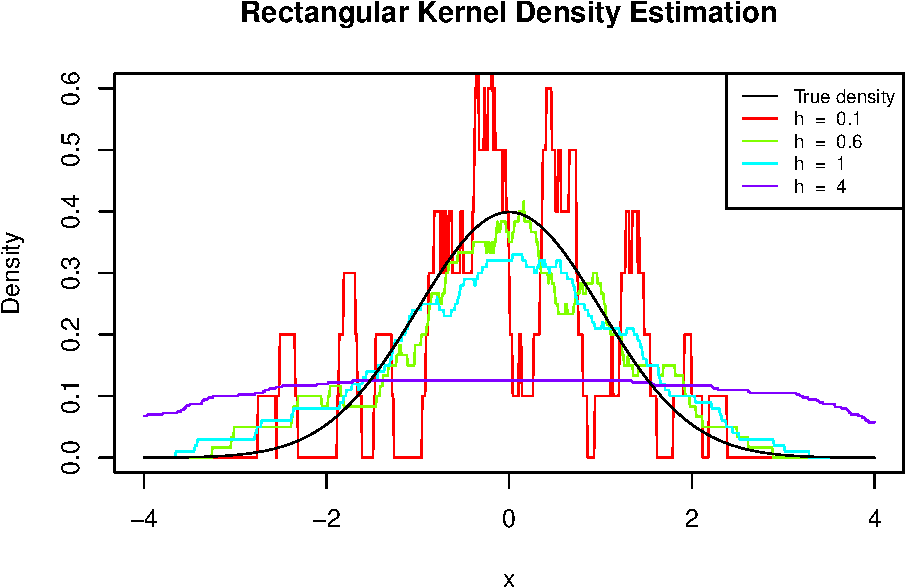
\includegraphics{project2_files/figure-latex/Kernel density estimation for standard normal-1.pdf}

\begin{Shaded}
\begin{Highlighting}[]
\CommentTok{# Gaussian kernel density estimation}
\KeywordTok{fnKernelPlot}\NormalTok{(x, X, fnGaussianKernel, h, }
             \DataTypeTok{title =} \StringTok{"Gaussian Kernel Density Estimation"}\NormalTok{,}
             \DataTypeTok{trueDensity =} \NormalTok{dnorm, }\DataTypeTok{ylim =} \KeywordTok{c}\NormalTok{(}\DecValTok{0}\NormalTok{, }\FloatTok{0.6}\NormalTok{))}
\end{Highlighting}
\end{Shaded}

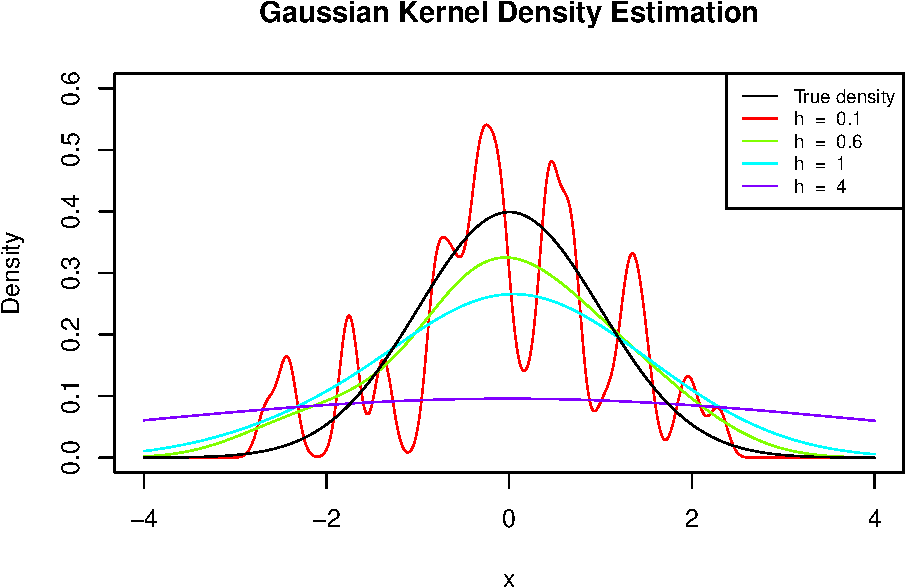
\includegraphics{project2_files/figure-latex/Kernel density estimation for standard normal-2.pdf}

\begin{Shaded}
\begin{Highlighting}[]
\CommentTok{# Epanechnikov kernel density estimation}
\KeywordTok{fnKernelPlot}\NormalTok{(x, X, fnEpanechnikovKernel, h, }
             \DataTypeTok{title =} \StringTok{"Epanechnikov Kernel Density Estimation"}\NormalTok{,}
             \DataTypeTok{trueDensity =} \NormalTok{dnorm, }\DataTypeTok{ylim =} \KeywordTok{c}\NormalTok{(}\DecValTok{0}\NormalTok{, }\FloatTok{0.6}\NormalTok{))}
\end{Highlighting}
\end{Shaded}

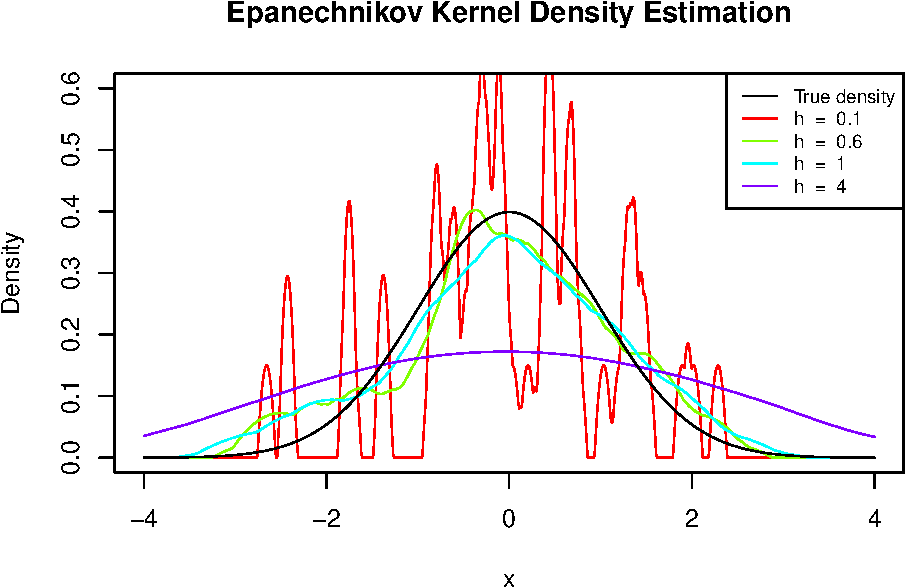
\includegraphics{project2_files/figure-latex/Kernel density estimation for standard normal-3.pdf}

Wir können sehen, dass die Wahl des Kerns die Glattheit der geschätzten
Dichtefunktion beeinflusst. Da der Rechteckskern sowie der
Epanechnikov-Kern den Träger \([-1,1]\) (bzw. \((-1,1)\)) besitzen,
finden sich Sprünge in den geschätzten Dichten. Da (mit \(h\) skalierte)
Differenzen in \([-1,1]\) für den Rechtseckskern gleich gewichtet
werden, sind die geschätzten Dichten nochmals sprunghafter im Vergleich
zum Epanechnikov-Kern, welcher symmetrisch um 0 monoton abfällt, was
eine Glättung zur Folge hat. Dabei nimmt die Sprunghöhe beim
Rechtseckskern mit steigender Bandbreite \(h\) ab. Im Vergleich dazu hat
der Gaußkern ganz \(\mathbb{R}\) als Träger und ist ebenso symmetrisch
um 0 monoton fallend. D.h.~für die Schätzung \(\hat{f}_n(x)\) an der
Stelle x hat jeder Datenpunkt \(X_i\), \(i = 1, \ldots,n\), einen (mit
wachsendem Abstand geringeren) Einfluss auf die Schätzung. Dadurch
resultieren glatte Kerndichteschätzer \(\hat{f}_n\).

Weiter können wir in den Beispielen schön das Bias-Varianz-Dilemma der
Bandweitenwahl beobachten. Für kleineres \(h\) wird die lokale Umgebung,
die für die Schätzung an der Stelle \(x\) herangezogen wird, ebenso
kleiner. Dies hat eine stärkere Oszillation der Schätzung \(\hat{f}_n\)
zur Folge. In diesem Fall ist der Bias klein (lokale Schätzung), die
Varianz jedoch hoch und das Resultat eine Unterglättung. Umgekehrt folgt
für eine größere Bandweite \(h\) ein größerer Bias (globale Schätzung),
jedoch eine geringere Varianz. In diesem Fall sprechen wir von
Überglättung. Die Aufgabe einer optimalen Bandweitenwahl ist es also
einen Ausgleich zwischen Bias und Varianz zu finden, so dass der
insgesamt resultierende Fehler möglichst minimal wird.

\subsubsection{Anwendung auf exponentialverteilte
Zufallszahlen}\label{anwendung-auf-exponentialverteilte-zufallszahlen}

\begin{Shaded}
\begin{Highlighting}[]
\CommentTok{# Generate sample}
\KeywordTok{set.seed}\NormalTok{(}\DecValTok{42}\NormalTok{)}
\NormalTok{n <-}\StringTok{ }\DecValTok{50}
\NormalTok{X <-}\StringTok{ }\KeywordTok{rexp}\NormalTok{(n)}

\CommentTok{# Define points to estimate kernel density on}
\NormalTok{x <-}\StringTok{ }\KeywordTok{seq}\NormalTok{(}\DecValTok{0}\NormalTok{, }\DecValTok{6}\NormalTok{, }\FloatTok{0.01}\NormalTok{)}

\CommentTok{# Set different bandwidths}
\NormalTok{h <-}\StringTok{ }\KeywordTok{c}\NormalTok{(}\FloatTok{0.1}\NormalTok{, }\FloatTok{0.5}\NormalTok{, }\DecValTok{1}\NormalTok{)}

\CommentTok{# Rectangular kernel density estimation}
\KeywordTok{fnKernelPlot}\NormalTok{(x, X, fnRectangularKernel, h, }
             \DataTypeTok{title =} \StringTok{"Rectangular Kernel Density Estimation"}\NormalTok{,}
             \DataTypeTok{trueDensity =} \NormalTok{dexp, }\DataTypeTok{ylim =} \KeywordTok{c}\NormalTok{(}\DecValTok{0}\NormalTok{, }\DecValTok{2}\NormalTok{))}
\end{Highlighting}
\end{Shaded}

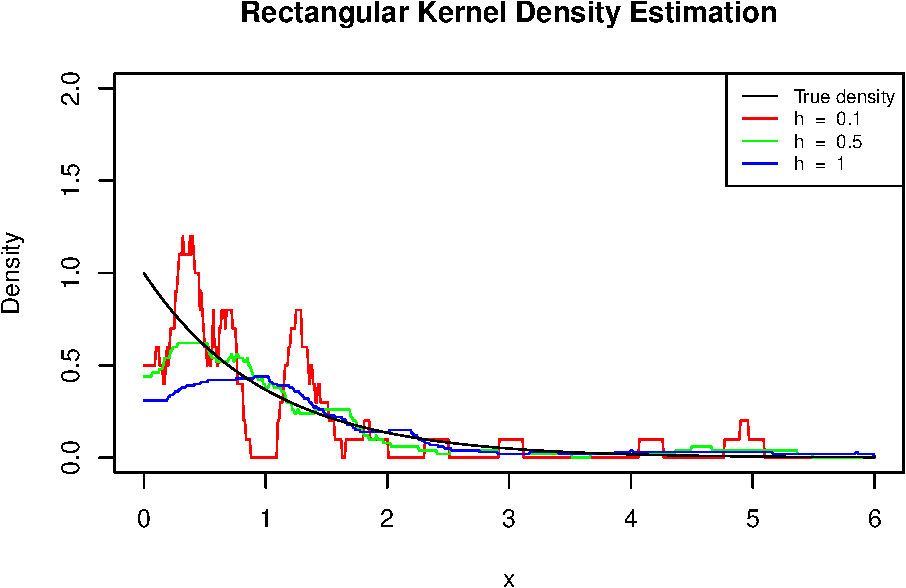
\includegraphics{project2_files/figure-latex/Kernel density estimation for the exponential-1.pdf}

\begin{Shaded}
\begin{Highlighting}[]
\CommentTok{# Gaussian kernel density estimation}
\KeywordTok{fnKernelPlot}\NormalTok{(x, X, fnGaussianKernel, h, }
             \DataTypeTok{title =} \StringTok{"Gaussian Kernel Density Estimation"}\NormalTok{,}
             \DataTypeTok{trueDensity =} \NormalTok{dexp, }\DataTypeTok{ylim =} \KeywordTok{c}\NormalTok{(}\DecValTok{0}\NormalTok{, }\DecValTok{2}\NormalTok{))}
\end{Highlighting}
\end{Shaded}

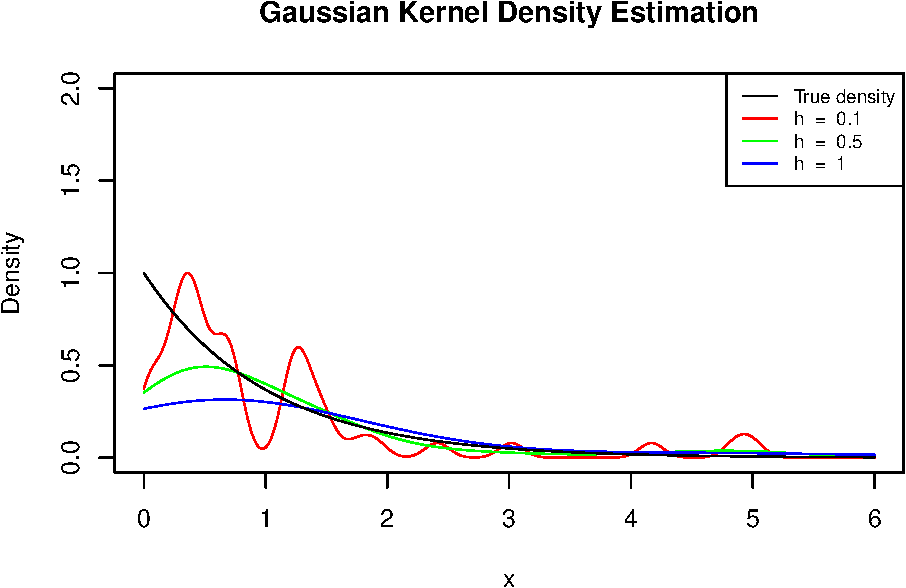
\includegraphics{project2_files/figure-latex/Kernel density estimation for the exponential-2.pdf}

\begin{Shaded}
\begin{Highlighting}[]
\CommentTok{# Epanechnikov kernel density estimation}
\KeywordTok{fnKernelPlot}\NormalTok{(x, X, fnEpanechnikovKernel, h, }
             \DataTypeTok{title =} \StringTok{"Epanechnikov Kernel Density Estimation"}\NormalTok{,}
             \DataTypeTok{trueDensity =} \NormalTok{dexp, }\DataTypeTok{ylim =} \KeywordTok{c}\NormalTok{(}\DecValTok{0}\NormalTok{, }\DecValTok{2}\NormalTok{))}
\end{Highlighting}
\end{Shaded}

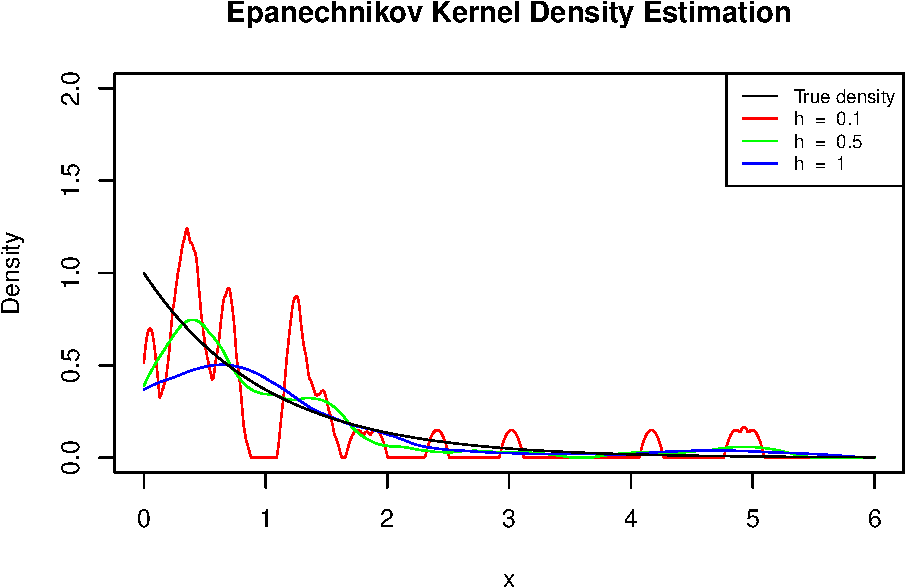
\includegraphics{project2_files/figure-latex/Kernel density estimation for the exponential-3.pdf}

Bei den Kerndichteschätzungen für exponentialverteilte Zufallszahlen
können wir ebenso den Einfluss der unterschiedlichen Kerne auf die
Glattheit der Schätzungen sowie das Bias-Varianz-Dilemma beobachten.
Insgesamt deuten die Kerndichteschätzungen auf eine rechtsschiefe
Verteilung hin, was in der Anwendung rechtsschiefe parametrische
Likelihood-Modelle (Exponentialverteilung, Log-Normalverteilung,
Chi-Quadrat-Verteilung, etc.) für die weitere Modellierung motivieren
könnte.

\subsubsection{Anwendung auf Cauchy-verteilte
Zufallszahlen}\label{anwendung-auf-cauchy-verteilte-zufallszahlen}

\begin{Shaded}
\begin{Highlighting}[]
\CommentTok{# Generate sample}
\KeywordTok{set.seed}\NormalTok{(}\DecValTok{42}\NormalTok{)}
\NormalTok{n <-}\StringTok{ }\DecValTok{50}
\NormalTok{X <-}\StringTok{ }\KeywordTok{rt}\NormalTok{(n, }\DataTypeTok{df =} \DecValTok{1}\NormalTok{)}

\CommentTok{# Define points to estimate kernel density on}
\NormalTok{x <-}\StringTok{ }\KeywordTok{seq}\NormalTok{(-}\DecValTok{5}\NormalTok{, }\DecValTok{5}\NormalTok{, }\FloatTok{0.01}\NormalTok{)}

\CommentTok{# Set different bandwidths}
\NormalTok{h <-}\StringTok{ }\KeywordTok{c}\NormalTok{(}\FloatTok{0.5}\NormalTok{, }\DecValTok{1}\NormalTok{, }\DecValTok{5}\NormalTok{)}

\CommentTok{# Define Cauchy density function}
\NormalTok{dcauchy <-}\StringTok{ }\NormalTok{function(x) \{y <-}\StringTok{ }\KeywordTok{dt}\NormalTok{(x, }\DataTypeTok{df =} \DecValTok{1}\NormalTok{)\}}

\CommentTok{# Rectangular kernel density estimation}
\KeywordTok{fnKernelPlot}\NormalTok{(x, X, fnRectangularKernel, h, }
             \DataTypeTok{title =} \StringTok{"Rectangular Kernel Density Estimation"}\NormalTok{,}
             \DataTypeTok{trueDensity =} \NormalTok{dcauchy, }\DataTypeTok{ylim =} \KeywordTok{c}\NormalTok{(}\DecValTok{0}\NormalTok{, }\FloatTok{0.4}\NormalTok{))}
\end{Highlighting}
\end{Shaded}

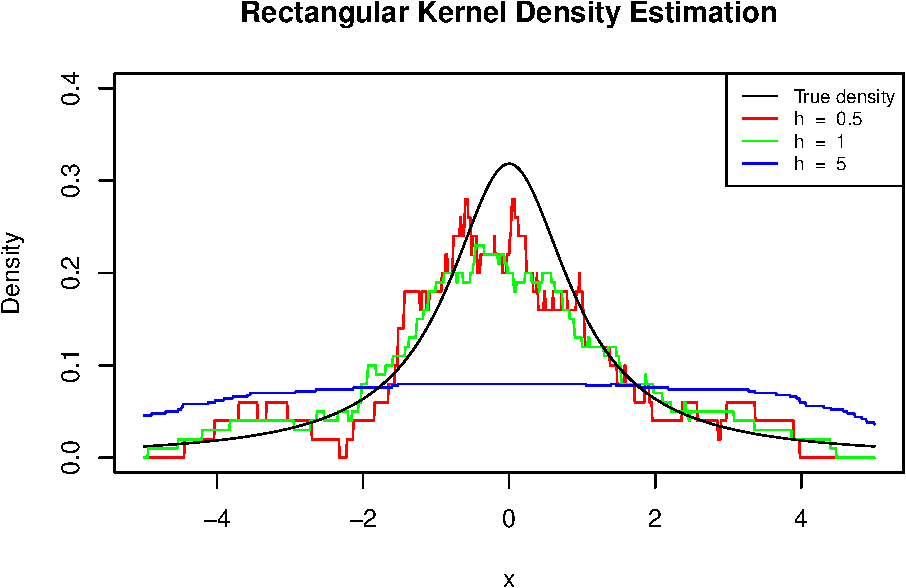
\includegraphics{project2_files/figure-latex/Kernel density estimation for Cauchy-1.pdf}

\begin{Shaded}
\begin{Highlighting}[]
\CommentTok{# Gaussian kernel density estimation}
\KeywordTok{fnKernelPlot}\NormalTok{(x, X, fnGaussianKernel, h, }
             \DataTypeTok{title =} \StringTok{"Gaussian Kernel Density Estimation"}\NormalTok{,}
             \DataTypeTok{trueDensity =} \NormalTok{dcauchy, }\DataTypeTok{ylim =} \KeywordTok{c}\NormalTok{(}\DecValTok{0}\NormalTok{, }\FloatTok{0.4}\NormalTok{))}
\end{Highlighting}
\end{Shaded}

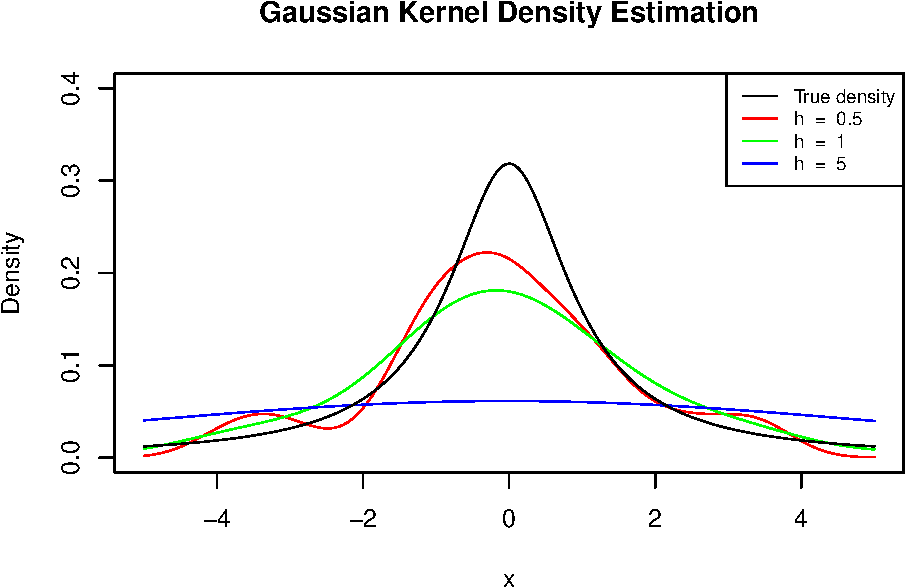
\includegraphics{project2_files/figure-latex/Kernel density estimation for Cauchy-2.pdf}

\begin{Shaded}
\begin{Highlighting}[]
\CommentTok{# Epanechnikov kernel density estimation}
\KeywordTok{fnKernelPlot}\NormalTok{(x, X, fnEpanechnikovKernel, h, }
             \DataTypeTok{title =} \StringTok{"Epanechnikov Kernel Density Estimation"}\NormalTok{,}
             \DataTypeTok{trueDensity =} \NormalTok{dcauchy, }\DataTypeTok{ylim =} \KeywordTok{c}\NormalTok{(}\DecValTok{0}\NormalTok{, }\FloatTok{0.4}\NormalTok{))}
\end{Highlighting}
\end{Shaded}

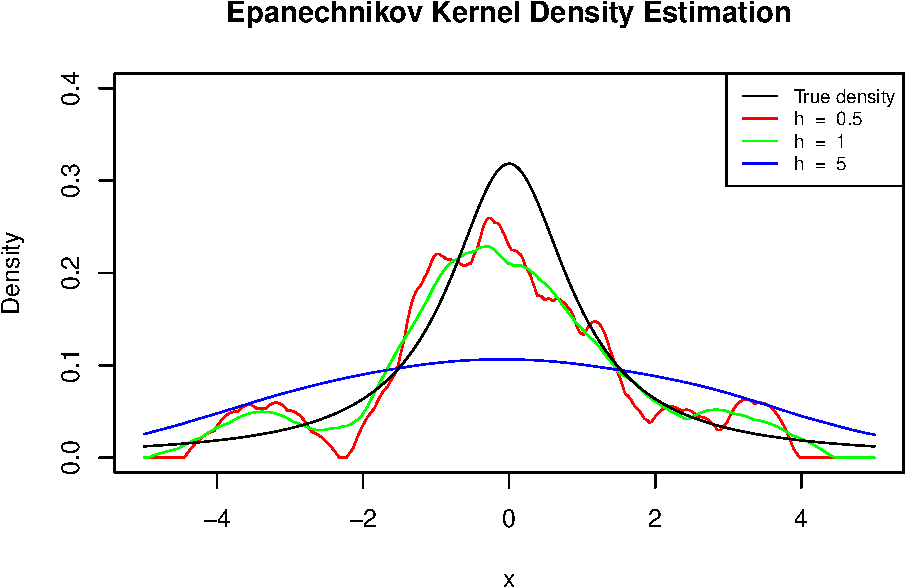
\includegraphics{project2_files/figure-latex/Kernel density estimation for Cauchy-3.pdf}

Auch hier können wir den Einfluss der unterschiedlichen Kerne auf die
Glattheit der Schätzungen sowie das Bias-Varianz-Dilemma beobachten.

\subsubsection{Anwendung auf faithful
Datensatz}\label{anwendung-auf-faithful-datensatz}

\begin{Shaded}
\begin{Highlighting}[]
\CommentTok{# Faithful kernel density estimation}
\NormalTok{X <-}\StringTok{ }\NormalTok{faithful$eruptions}

\CommentTok{# Define points to estimate kernel density on}
\NormalTok{x <-}\StringTok{ }\KeywordTok{seq}\NormalTok{(}\KeywordTok{min}\NormalTok{(X), }\KeywordTok{max}\NormalTok{(X), }\FloatTok{0.01}\NormalTok{)}

\CommentTok{# Set different bandwidths}
\NormalTok{h <-}\StringTok{ }\KeywordTok{c}\NormalTok{(}\FloatTok{0.05}\NormalTok{, }\KeywordTok{bw.ucv}\NormalTok{(X), }\FloatTok{0.5}\NormalTok{, }\DecValTok{1}\NormalTok{)}

\CommentTok{# Gaussian kernel density estimation}
\NormalTok{title <-}\StringTok{ "Gaussian Kernel Density Estimation for faithful eruption data"}
\KeywordTok{fnKernelPlot}\NormalTok{(x, X, fnGaussianKernel, h, }\DataTypeTok{title =} \NormalTok{title)}
\end{Highlighting}
\end{Shaded}

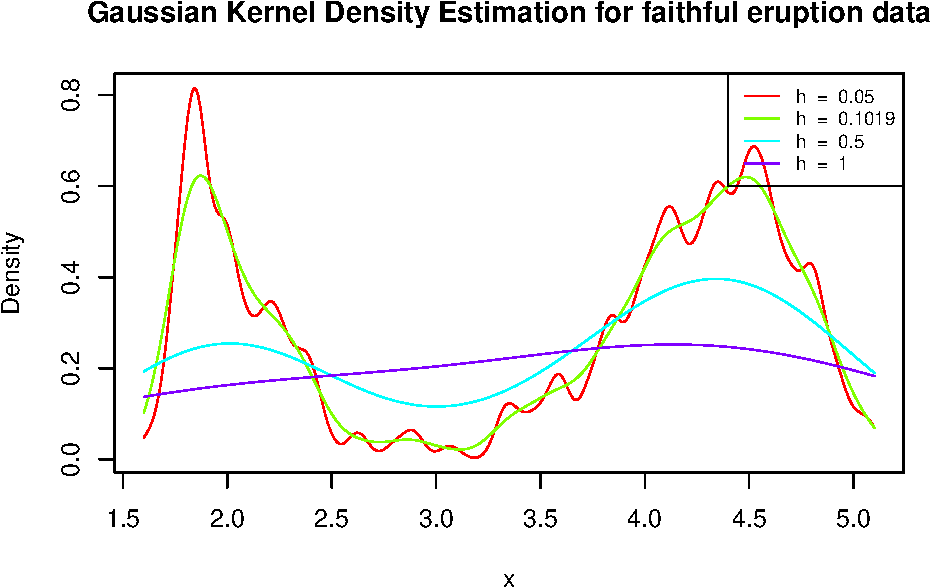
\includegraphics{project2_files/figure-latex/faithful kernel density estimation-1.pdf}

Wir können sehen, dass die Anwendung des Kerndichteschätzers mit
Gaußkern für verschiedene Bandweiten eine bimodale Verteilung der
Eruptionsdauern im Datensatz \texttt{faithful} aufzeigt, was auf zwei
unterschiedliche Gruppen von Ausstößen hindeutet.

\subsection{Kreuzvalidierung zur
Bandweitenwahl}\label{kreuzvalidierung-zur-bandweitenwahl}

Die Idee der Kreuzvalidierung ist es die Bandweite \(h\) so zu wählen,
dass der Mean Integrated Squared Error (MISE) minimal wird. Es gilt:

\[
\begin{aligned}
\argmin_h \text{MISE}(h) &= \argmin_h \mathbb{E} \left[ \int (\hat{f}_n(x) - f(x))^2 \, dx \right] \\
&= \argmin_h \mathbb{E} \left[ \int \hat{f}_n^2(x) \, dx - 2 \int \hat{f}_n(x) f(x) \, dx \right] + \int f^2(x) \, dx \\
&= \argmin_h \mathbb{E} \left[ \int \hat{f}_n^2(x) \, dx - 2 \int \hat{f}_n(x) f(x) \, dx \right] = \argmin_h J(h)
\end{aligned}
\]

mit \(J\) definiert durch

\[
J(h) := \mathbb{E} \left[ \int \hat{f}_n^2(x) \, dx - 2 \int \hat{f}_n(x) f(x) \, dx \right] , \quad h >0.
\]

\subsubsection{\texorpdfstring{Erwartungstreue des
Kreuzvalidierungskriteriums
\(\hat{J}(h)\)}{Erwartungstreue des Kreuzvalidierungskriteriums \textbackslash{}hat\{J\}(h)}}\label{erwartungstreue-des-kreuzvalidierungskriteriums-hatjh}

Wir zeigen nun, dass das Kreuzvalidierungskriterium \(\hat{J}(h)\)
definiert durch \[
\hat{J}(h) := \int \hat{f}_n^2(x) \, dx - 2 \hat{G}, \quad h >0,
\] mit \[
\hat{G} := \frac{1}{n} \sum_{j=1}^n \hat{f}_{n,-j}(X_j), \quad \hat{f}_{n,-j}(x) := \frac{1}{(n-1)h} \sum_{k\not=j} K\left( \frac{X_k-x}{h} \right)
\] ein erwartungstreuer Schätzer für \(J(h)\) ist.

Seien \(X_1, \ldots, X_n \overset{iid}{\sim} \mathbb{P}_f\) und
betrachte für \(h>0\) und \(j \in \{1, \ldots,n\}\) \[
\begin{aligned}
\mathbb{E}\left[ \hat{f}_{n,-j}(X_j) \right] &= \mathbb{E}\left[ \frac{1}{(n-1)h} \sum_{k\not=j} K\left( \frac{X_k-X_j}{h} \right) \right] \\
&\overset{iid}{=} \frac{1}{(n-1)h} \sum_{k\not=j} \int \int K\left( \frac{y-x}{h} \right) f(y) \, dy \, f(x) \, dx \\
&= \frac{1}{h} \int \int K\left( \frac{y-x}{h} \right) f(y) \, dy \, f(x) \, dx \\
&= \int \int K(y) f(x+hy) \, dy \, f(x) \, dx.
\end{aligned}
\] Ebenso gilt \[
\begin{aligned}
\mathbb{E} \left[ \int \hat{f}_n(x) f(x) \, dx \right] &= \mathbb{E} \left[ \int \frac{1}{nh} \left( \sum_{k=1}^n K\left( \frac{X_k-x}{h} \right) \right) f(x) \, dx \right] \\
&\overset{\text{Fubini}}{=} \frac{1}{nh} \sum_{k=1}^n \int \mathbb{E} \left[ K\left( \frac{X_k-x}{h} \right) \right] f(x) \, dx \\
&\overset{iid}{=} \frac{1}{h} \int \mathbb{E} \left[ K\left( \frac{X_1-x}{h} \right) \right] f(x) \, dx \\
&= \int \int K(y) f(x+hy) \, dy \, f(x) \, dx.
\end{aligned}
\]

Somit folgt also \[
\begin{aligned}
\mathbb{E} [\hat{J}(h)] &= \mathbb{E} \left[ \int \hat{f}_n^2(x) \, dx - 2 \hat{G} \right] \\
&= \mathbb{E} \left[ \int \hat{f}_n^2(x) \, dx \right] - 2 \mathbb{E}[\hat{G}] \\
&= \mathbb{E} \left[ \int \hat{f}_n^2(x) \, dx \right] - 2 \mathbb{E}\left[ \frac{1}{n} \sum_{j=1}^n \hat{f}_{n,-j}(X_j) \right] \\
&\overset{iid}{=} \mathbb{E} \left[ \int \hat{f}_n^2(x) \, dx \right] - 2 \mathbb{E}\left[ \hat{f}_{n,-1}(X_1) \right] \\
&= \mathbb{E} \left[ \int \hat{f}_n^2(x) \, dx - 2 \int \hat{f}_n(x) f(x) \, dx \right] = J(h).
\end{aligned}
\] Aus dieser Herleitung sind auch die notwendigen
Integrationsbedingungen an \(K\) und \(f\) erkennbar. Damit
\(\mathbb{E}[\hat{G}] < \infty\), muss für \(h>0\) also
\(y \mapsto K(y)f(x+hy) \in \mathcal{L}^1(\mathbb{R}, \mathcal{B}(\mathbb{R}), \lambda)\)
für jedes \(x \in \mathbb{R}\) gelten. Betrachten wir \[
\begin{aligned}
\mathbb{E} \left[ \int \hat{f}_n^2(x) \, dx \right] &= \mathbb{E} \left[ \frac{1}{(nh)^2} \int \left( \sum_{k=1}^n K\left( \frac{X_k-x}{h} \right) \right)^2 \, dx \right] \\
&\overset{\text{Fubini}}{=} \frac{1}{(nh)^2} \int \mathbb{E} \left[ \left( \sum_{k=1}^n K\left( \frac{X_k-x}{h} \right) \right)^2 \right] \, dx \\
&= \frac{1}{(nh)^2} \left\{ \sum_{k=1}^n \int \mathbb{E} \left[ K^2\left( \frac{X_k-x}{h} \right) \right] \, dx + 2 \sum_{k \not= j} \int \mathbb{E} \left[ K\left( \frac{X_k-x}{h} \right) K\left( \frac{X_j-x}{h} \right) \right] \, dx \right\} \\
&\overset{iid}{=} \frac{1}{nh} \int K^2(y) f(x+hy) \, dy \, dx + \frac{2(n-1)}{n^2} \int \left( \int K(y) f(x+hy) \, dy \right)^2 \, dx
\end{aligned}
\] so können wir weiter sehen, dass die quadratische Integrationsannahme
\(y \mapsto K^2(y) f(x+hy) \in \mathcal{L}^1(\mathbb{R}, \mathcal{B}(\mathbb{R}), \lambda)\)
für alle \(x \in \mathbb{R}\) ebenso erfüllt sein muss, damit
\(\mathbb{E}[\hat{J}(h)]\) für \(h>0\) existiert.

\subsubsection{Implementierung der Kreuzvalidierung zur
Bandweitenwahl}\label{implementierung-der-kreuzvalidierung-zur-bandweitenwahl}

Wir implementieren die Kreuzvalidierung in zwei Schritten: wir schreiben
erstens eine Funktion \texttt{fnJ} die das Kreuzvalidierungskriterium
\(\hat{J}(h)\) berechnet und zweitens eine Funktion \texttt{fnUCV} die
dann das Kreuzvalidierungskriterium minimiert. Um das Integral über den
quadratischen Kerndichteschätzer zu berechnen nutzen wir die R-Methode
\texttt{integrate}. Für die Minimierung in \texttt{fnUCV} bedinen wir
uns der R-Methode \texttt{optimize}.

\begin{Shaded}
\begin{Highlighting}[]
\NormalTok{fnJ <-}\StringTok{ }\NormalTok{function(X, K, h) \{}
  \CommentTok{# This function computes the value of the unbiased cross validation criteria.}
  \CommentTok{# The minimum of this function in h gives an estimated “optimal” (in the}
  \CommentTok{# sense of mean integrated squared error) bandwidth.}
  \CommentTok{# }
  \CommentTok{# Args:}
  \CommentTok{#   X: Data sample on which the kernel density estimation is fitted}
  \CommentTok{#   K: Kernel function to be used for smoothing}
  \CommentTok{#   h: Smoothing bandwidth}
  \CommentTok{#   }
  \CommentTok{# Returns:}
  \CommentTok{#   Function value}
  
  \NormalTok{n <-}\StringTok{ }\KeywordTok{length}\NormalTok{(X)}
  
  \CommentTok{# Compute integral of squared kernel density estimator}
  \NormalTok{integrand <-}\StringTok{ }\NormalTok{function(x) \{}\KeywordTok{return}\NormalTok{(}\KeywordTok{fnKernelDensityEst}\NormalTok{(x, X, K, h)^}\DecValTok{2}\NormalTok{)\}}
  \NormalTok{SKDEInt <-}\StringTok{ }\KeywordTok{integrate}\NormalTok{(integrand, -}\OtherTok{Inf}\NormalTok{, }\OtherTok{Inf}\NormalTok{)$value}
  
  \CommentTok{# Compute G}
  \NormalTok{mKernels <-}\StringTok{ }\KeywordTok{K}\NormalTok{((}\DecValTok{1}\NormalTok{/h) *}\StringTok{ }\KeywordTok{outer}\NormalTok{(X, X, }\DataTypeTok{FUN =} \StringTok{"-"}\NormalTok{))}
  \KeywordTok{diag}\NormalTok{(mKernels) <-}\StringTok{ }\DecValTok{0}
  \NormalTok{G <-}\StringTok{ }\NormalTok{(}\DecValTok{1}\NormalTok{/(n*(n}\DecValTok{-1}\NormalTok{)*h)) *}\StringTok{ }\KeywordTok{sum}\NormalTok{(mKernels)}
  
  \CommentTok{# Return function value of J}
  \KeywordTok{return}\NormalTok{(SKDEInt -}\StringTok{ }\DecValTok{2}\NormalTok{*G)}
\NormalTok{\}}

\NormalTok{fnUCV <-}\StringTok{ }\NormalTok{function(X, K, hmin, hmax, }\DataTypeTok{tol =} \FloatTok{0.1} \NormalTok{*}\StringTok{ }\NormalTok{hmin) \{}
  \CommentTok{# This function returns the minimum of the unbiased cross validation criteria}
  \CommentTok{# in h which is “optimal” in the sense of mean integrated squared error.}
  \CommentTok{# We use R's optimize function to find the minimum.}
  \CommentTok{# }
  \CommentTok{# Args:}
  \CommentTok{#   X:    Data sample on which the kernel density estimation is fitted}
  \CommentTok{#   K:    Kernel function to be used for smoothing}
  \CommentTok{#   hmin: Lower bound for optimal h}
  \CommentTok{#   hmax: Upper bound for optimal h}
  \CommentTok{#   tol:  The desired accuracy}
  \CommentTok{#   }
  \CommentTok{# Returns:}
  \CommentTok{#   Optimal bandwidth h*}
  
  \CommentTok{# Find and return the minimum using optimize}
  \NormalTok{fnTarget <-}\StringTok{ }\NormalTok{function(h) \{}\KeywordTok{return}\NormalTok{(}\KeywordTok{fnJ}\NormalTok{(X, K, h))\}}
  \NormalTok{hOpt <-}\StringTok{ }\KeywordTok{optimize}\NormalTok{(fnTarget, }\KeywordTok{c}\NormalTok{(hmin, hmax), }\DataTypeTok{tol =} \NormalTok{tol)}
  \KeywordTok{return}\NormalTok{(hOpt$minimum)}
\NormalTok{\}}
\end{Highlighting}
\end{Shaded}

Wir berechnen nun mit unserer Implementierung der Kreuzvalidierung die
optimale Bandweite \(h^*\) für die bereits zuvor betrachteten
Eruptionsdauern im Datensatz \texttt{faithful}. Für den
Kerndichteschätzer wählen wir einen Gaußkern:

\begin{Shaded}
\begin{Highlighting}[]
\NormalTok{hmin <-}\StringTok{ }\FloatTok{0.01}
\NormalTok{hmax <-}\StringTok{ }\DecValTok{10}
\KeywordTok{fnUCV}\NormalTok{(faithful$eruptions, fnGaussianKernel, hmin, hmax)}
\end{Highlighting}
\end{Shaded}

\begin{verbatim}
## [1] 0.102756
\end{verbatim}

Vergleichen wir dieses Ergebnis mit der optimalen Bandweite gemäß der
R-Methode \texttt{bw.ucv} (bandwidth unbiased cross validation), so
erhalten wir ein sehr ähnliches Ergebnis:

\begin{Shaded}
\begin{Highlighting}[]
\KeywordTok{bw.ucv}\NormalTok{(faithful$eruptions)}
\end{Highlighting}
\end{Shaded}

\begin{verbatim}
## [1] 0.1019193
\end{verbatim}

Es ist anzunehmen, dass die Implementierung der erwartungstreuen
Kreuzvalidierung in \texttt{bw.ucv} effizienter ist als unsere, da die
R-Methode nur für einen Gaußkern implementiert ist, d.h.~hierfür
ggf.~analytische Möglichkeiten ausgenutzt wurden. Im Vergleich dazu
besteht in unserer Implementierung die Möglichkeit weitere Kerne
anzuwenden.

\subsection{\texorpdfstring{\(m\)-nächste
Nachbarn}{m-nächste Nachbarn}}\label{m-nachste-nachbarn}

Zusätzlich zur Kerndichteschätzung mit fixer Bandweite \(h > 0\) wollen
wir die \(m\)-nächste Nachbarn Methode mit variabler Bandweite
implementieren. Für eine Stelle \(x \in \mathbb{R}\) ist die Bandweite
\(h(x,m)\) bei der \(knn(m)\)-Methode durch den Abstand von \(x\) zum
\(m\)-nächsten Nachbarn definiert.

\begin{Shaded}
\begin{Highlighting}[]
\NormalTok{fnMNearestNeighbors <-}\StringTok{ }\NormalTok{function(x, X, K, m) \{}
  \CommentTok{# This function computes the kernel density estimates for a given sample X and}
  \CommentTok{# kernel K with variable bandwidths h for every point, which are determined by}
  \CommentTok{# the m-nearest neighbor approach}
  \CommentTok{# }
  \CommentTok{# Args:}
  \CommentTok{#   x: Points for which the kernel density estimates are computed}
  \CommentTok{#   X: Data sample on which the kernel density estimation is fitted}
  \CommentTok{#   K: Kernel function to be used for smoothing}
  \CommentTok{#   m: Neighbor position}
  \CommentTok{#   }
  \CommentTok{# Returns:}
  \CommentTok{#   A vector of the nearest neighbor kernel density estimates at points x}
  
  \NormalTok{n <-}\StringTok{ }\KeywordTok{length}\NormalTok{(X)}
  
  \CommentTok{# Compute bandwidth for every point x}
  \NormalTok{h <-}\StringTok{ }\KeywordTok{apply}\NormalTok{(}\KeywordTok{abs}\NormalTok{(}\KeywordTok{outer}\NormalTok{(X, x, }\StringTok{"-"}\NormalTok{)), }\DecValTok{2}\NormalTok{, sort)[m,]}
  
  \CommentTok{# Compute kernel density estimation values using outer}
  \NormalTok{mKernels <-}\StringTok{ }\KeywordTok{K}\NormalTok{((}\DecValTok{1}\NormalTok{/}\KeywordTok{t}\NormalTok{(}\KeywordTok{matrix}\NormalTok{(}\KeywordTok{rep}\NormalTok{(h, n), }\DataTypeTok{ncol =} \NormalTok{n))) *}\StringTok{ }\KeywordTok{outer}\NormalTok{(X, x, }\DataTypeTok{FUN =} \StringTok{"-"}\NormalTok{))}
  \KeywordTok{return}\NormalTok{((}\DecValTok{1}\NormalTok{/(n*h)) *}\StringTok{ }\KeywordTok{colSums}\NormalTok{(mKernels))}
\NormalTok{\}}
\end{Highlighting}
\end{Shaded}

Betrachten wir die \(knn(m)\)-Schätzungen für standard-normalverteilte
Daten wiederum für den Rechteckskern, Gaußkern sowie Epanechnikov-Kern
für verschiedene \(m\):

\begin{Shaded}
\begin{Highlighting}[]
\CommentTok{# Generate sample}
\KeywordTok{set.seed}\NormalTok{(}\DecValTok{42}\NormalTok{)}
\NormalTok{n <-}\StringTok{ }\DecValTok{50}
\NormalTok{X <-}\StringTok{ }\KeywordTok{rnorm}\NormalTok{(n)}

\CommentTok{# Define points to estimate kernel density on}
\NormalTok{x <-}\StringTok{ }\KeywordTok{seq}\NormalTok{(-}\DecValTok{4}\NormalTok{, }\DecValTok{4}\NormalTok{, }\FloatTok{0.01}\NormalTok{)}

\CommentTok{# Define vector of neighbor positions m}
\NormalTok{m <-}\StringTok{ }\KeywordTok{c}\NormalTok{(}\DecValTok{5}\NormalTok{,}\DecValTok{10}\NormalTok{,}\DecValTok{25}\NormalTok{,}\DecValTok{40}\NormalTok{,}\DecValTok{50}\NormalTok{)}

\CommentTok{# Nearest Neighbor Rectangular kernel density estimation}
\KeywordTok{fnKernelPlot}\NormalTok{(x, X, fnRectangularKernel, }\DataTypeTok{vm =} \NormalTok{m,}
             \DataTypeTok{fnEstimation =} \NormalTok{fnMNearestNeighbors,}
             \DataTypeTok{title =} \StringTok{"Nearest Neighbor Rectangular Kernel Density Estimation"}\NormalTok{,}
             \DataTypeTok{trueDensity =} \NormalTok{dnorm, }\DataTypeTok{ylim =} \KeywordTok{c}\NormalTok{(}\DecValTok{0}\NormalTok{, }\FloatTok{0.6}\NormalTok{))}
\end{Highlighting}
\end{Shaded}

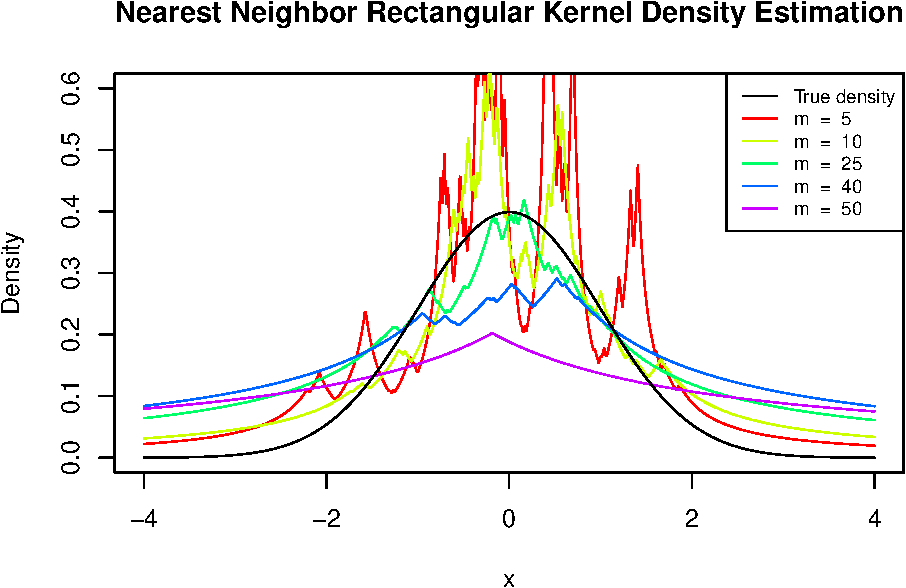
\includegraphics{project2_files/figure-latex/m-nearest neighbors test-1.pdf}

\begin{Shaded}
\begin{Highlighting}[]
\CommentTok{# Nearest Neighbor Gaussian kernel density estimation}
\KeywordTok{fnKernelPlot}\NormalTok{(x, X, fnGaussianKernel, }\DataTypeTok{vm =} \NormalTok{m, }
             \DataTypeTok{fnEstimation =} \NormalTok{fnMNearestNeighbors,}
             \DataTypeTok{title =} \StringTok{"Nearest Neighbor Gaussian Kernel Density Estimation"}\NormalTok{,}
             \DataTypeTok{trueDensity =} \NormalTok{dnorm, }\DataTypeTok{ylim =} \KeywordTok{c}\NormalTok{(}\DecValTok{0}\NormalTok{, }\FloatTok{0.6}\NormalTok{))}
\end{Highlighting}
\end{Shaded}

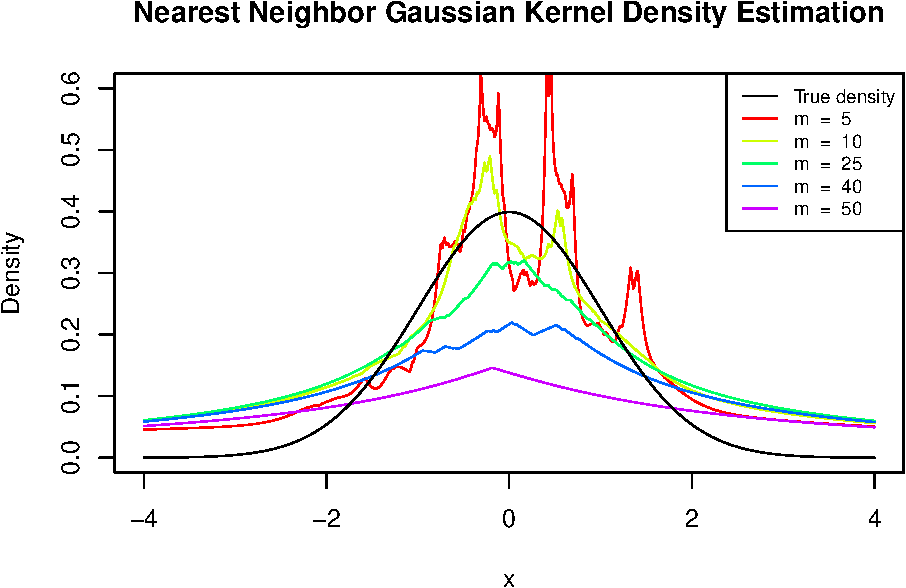
\includegraphics{project2_files/figure-latex/m-nearest neighbors test-2.pdf}

\begin{Shaded}
\begin{Highlighting}[]
\CommentTok{# Nearest Neighbor Epanechnikov kernel density estimation}
\KeywordTok{fnKernelPlot}\NormalTok{(x, X, fnEpanechnikovKernel, }\DataTypeTok{vm =} \NormalTok{m, }
             \DataTypeTok{fnEstimation =} \NormalTok{fnMNearestNeighbors, }
             \DataTypeTok{title =} \StringTok{"Nearest Neighbor Epanechnikov Kernel Density Estimation"}\NormalTok{,}
             \DataTypeTok{trueDensity =} \NormalTok{dnorm, }\DataTypeTok{ylim =} \KeywordTok{c}\NormalTok{(}\DecValTok{0}\NormalTok{, }\FloatTok{0.6}\NormalTok{))}
\end{Highlighting}
\end{Shaded}

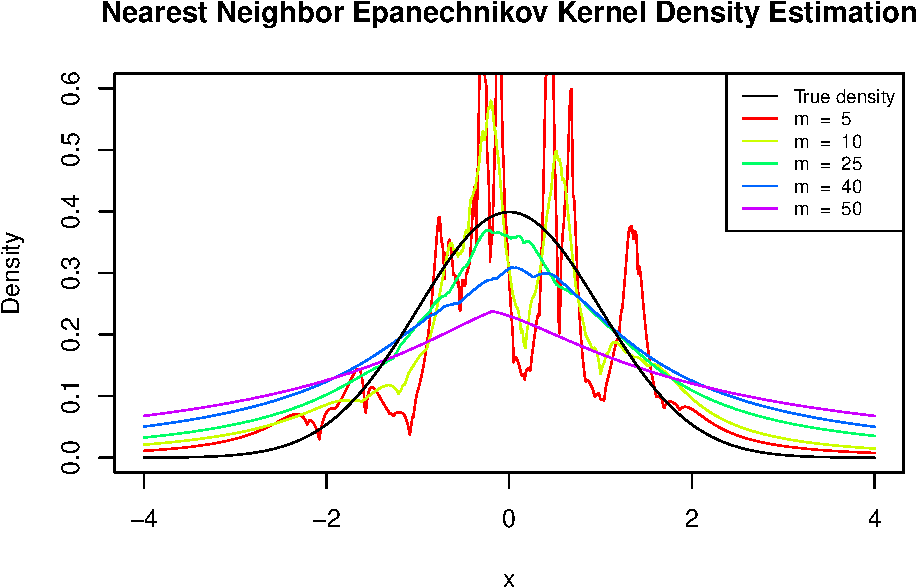
\includegraphics{project2_files/figure-latex/m-nearest neighbors test-3.pdf}

Im Vergleich zur Kerndichteschätzung mit fixer Bandweite \(h>0\) passt
die \(knn(m)\)-Methode die Bandweite in Abhängigkeit des Abstands der
Stelle \(x\) zu den \(m\)-nächsten Datenpunkten aus \(X_1, \ldots, X_n\)
variabel an. Dies hat zur Folge, dass die Bandweiten zu \(x\) in
Umgebungen, in welchen sich Datenpunkte häufen, kleiner gewählt werden
und somit lokaler geschätzt wird. Dagegen wird für Stellen \(x\), für
welche die Umgebung zum \(m\)-nächsten Nachbarn groß ist eine größere
Bandweite gewählt, was eine globalere Schätzung zur Folge hat. Diese
Überlegung wird in den Plots bestätigt. In kleineren Umgebungen um 0, in
welchen sich die standard-normalverteilten Zufallszahlen häufen,
oszillieren die \(knn(m)\)-Schätzungen stärker als in den Tails. Damit
wird tendenziell in kleineren Umgebungen um 0 unterglättet und in den
Tails überglättet. Weiter lässt sich wie zu erwarten erkennen, dass mit
größerem \(m\) die Schätzungen glatter werden, da für größeres \(m\) die
Bandweiten \(h(x,m)\) für alle Stellen \(x\) verhältnismäßig größer
werden.

Insgesamt ist im Vergleich zur Kerndichteschätzung mit fixer Bandweite
\(h>0\) tendenziell eine stärkere Oszillation der Schätzungen
festzustellen.

\section{Bildentrauschen}\label{bildentrauschen}

In dieser Aufgabe wollen wir mit Hilfe des Nadaraya-Watson-Schätzers
versuchen Bilder zu entrauschen. Zunächst laden wir das Bild
\texttt{lena.png} und wandeln es in Graustufen um:

\begin{Shaded}
\begin{Highlighting}[]
\CommentTok{# Load package}
\KeywordTok{library}\NormalTok{(EBImage)}

\CommentTok{# Load image from parent directory}
\NormalTok{imgLenaColor <-}\StringTok{ }\KeywordTok{readImage}\NormalTok{(}\StringTok{"lena.png"}\NormalTok{)}

\CommentTok{# Change image to grayscale}
\NormalTok{imgLenaGray <-}\StringTok{ }\KeywordTok{channel}\NormalTok{(imgLenaColor, }\StringTok{"gray"}\NormalTok{)}

\CommentTok{# Display images}
\KeywordTok{par}\NormalTok{(}\DataTypeTok{mfrow =} \KeywordTok{c}\NormalTok{(}\DecValTok{1}\NormalTok{,}\DecValTok{2}\NormalTok{))}
\KeywordTok{display}\NormalTok{(imgLenaColor, }\DataTypeTok{method =} \StringTok{"raster"}\NormalTok{)}
\KeywordTok{display}\NormalTok{(imgLenaGray, }\DataTypeTok{method =} \StringTok{"raster"}\NormalTok{)}
\end{Highlighting}
\end{Shaded}

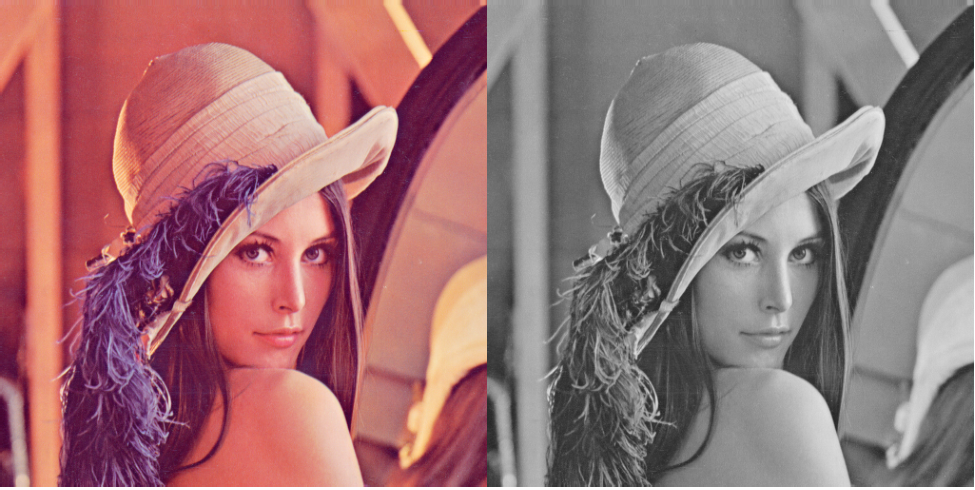
\includegraphics{project2_files/figure-latex/Load and prepare images-1.pdf}

Als nächstes implementieren wir eine Funktion die es uns ermöglicht ein
verrauschtes Bild zu erzeugen, wobei die Verteilung des Rauschens sowie
das Rauschniveau spezifiziert werden kann:

\begin{Shaded}
\begin{Highlighting}[]
\NormalTok{fnAddNoise <-}\StringTok{ }\NormalTok{function(img, rnoise, ...) \{}
  \CommentTok{# This function adds noise specified by rnoise to a grayscale image. If the}
  \CommentTok{# image is not grayscale, it gets converted to grayscale first.}
  \CommentTok{# }
  \CommentTok{# Args:}
  \CommentTok{#   img:    Image}
  \CommentTok{#   rnoise: Random noise generation function (e.g. rnorm for Gaussian noise)}
  \CommentTok{#   ...:    Further arguments passed to or from other methods}
  \CommentTok{#   }
  \CommentTok{# Returns:}
  \CommentTok{#   Grayscale image with added noise}
  
  \CommentTok{# Check if grayscale and convert if necessary}
  \NormalTok{if(}\KeywordTok{colorMode}\NormalTok{(img) !=}\StringTok{ }\DecValTok{0}\NormalTok{) \{img <-}\StringTok{ }\KeywordTok{channel}\NormalTok{(img, }\StringTok{"gray"}\NormalTok{)\}}
  
  \CommentTok{# Add noise}
  \NormalTok{m <-}\StringTok{ }\KeywordTok{dim}\NormalTok{(img)[}\DecValTok{1}\NormalTok{]}
  \NormalTok{p <-}\StringTok{ }\KeywordTok{dim}\NormalTok{(img)[}\DecValTok{2}\NormalTok{]}
  \NormalTok{imgNoise <-}\StringTok{ }\KeywordTok{Image}\NormalTok{(}\KeywordTok{imageData}\NormalTok{(img) +}\StringTok{ }\KeywordTok{matrix}\NormalTok{(}\KeywordTok{rnoise}\NormalTok{(m*p, ...), m, p))}
  
  \CommentTok{# Adjust values below 0 and above 1}
  \NormalTok{imgNoise[imgNoise <}\StringTok{ }\DecValTok{0}\NormalTok{] <-}\StringTok{ }\DecValTok{0}
  \NormalTok{imgNoise[imgNoise >}\StringTok{ }\DecValTok{1}\NormalTok{] <-}\StringTok{ }\DecValTok{1}
  
  \KeywordTok{return}\NormalTok{(imgNoise)}
\NormalTok{\}}
\end{Highlighting}
\end{Shaded}

Betrachten wir drei verrauschte Bilder mit Gaußschem Rauschen für
unterschiedliche Rauschniveaus:

\begin{Shaded}
\begin{Highlighting}[]
\NormalTok{imgLenaNoise1 <-}\StringTok{ }\KeywordTok{fnAddNoise}\NormalTok{(imgLenaGray, rnorm, }\DataTypeTok{sd =} \FloatTok{0.1}\NormalTok{)}
\NormalTok{imgLenaNoise2 <-}\StringTok{ }\KeywordTok{fnAddNoise}\NormalTok{(imgLenaGray, rnorm, }\DataTypeTok{sd =} \FloatTok{0.25}\NormalTok{)}
\NormalTok{imgLenaNoise3 <-}\StringTok{ }\KeywordTok{fnAddNoise}\NormalTok{(imgLenaGray, rnorm, }\DataTypeTok{sd =} \FloatTok{0.5}\NormalTok{)}

\KeywordTok{par}\NormalTok{(}\DataTypeTok{mfrow =} \KeywordTok{c}\NormalTok{(}\DecValTok{1}\NormalTok{,}\DecValTok{3}\NormalTok{))}
\KeywordTok{display}\NormalTok{(imgLenaNoise1, }\DataTypeTok{method =} \StringTok{"raster"}\NormalTok{)}
\KeywordTok{display}\NormalTok{(imgLenaNoise2, }\DataTypeTok{method =} \StringTok{"raster"}\NormalTok{)}
\KeywordTok{display}\NormalTok{(imgLenaNoise3, }\DataTypeTok{method =} \StringTok{"raster"}\NormalTok{)}
\end{Highlighting}
\end{Shaded}

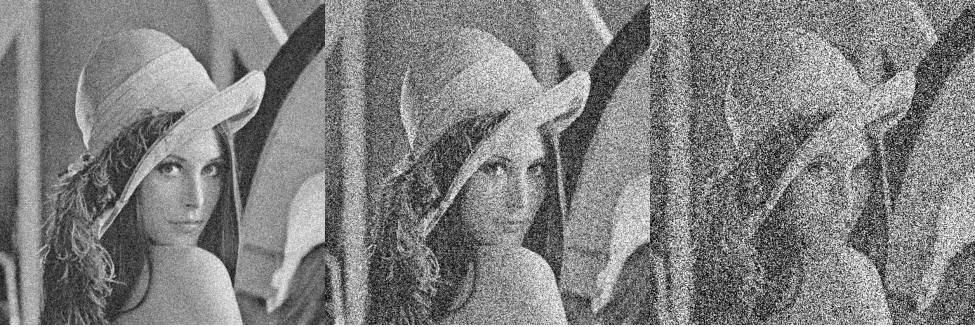
\includegraphics{project2_files/figure-latex/Noise Example-1.pdf}

\subsection{Nadaraya-Watson-Schätzer}\label{nadaraya-watson-schatzer}

In diesem Abschnitt wollen wir einen geeigneten Nadaraya-Watson-Schätzer
zur Bildentrauschung angeben sowie effizient implementieren.

Dazu zeigen wir zunächst, dass
\(K_2(x,y) := K(x)K(y), \, x,y, \in \mathbb{R}\) für einen
eindimensionalen Kern \(K\) einen zweidimensionalen Kern definiert: Da
\(K\) ein eindimensionaler Kern ist, ist \(K\) eine nichtnegative,
reelle Funktion mit \[
\int K(y) \, dy = 1 \quad \text{und} \quad K(x) = K(-x) \, \text{ für alle } x\in \mathbb{R}.
\]

Damit ist \(K_2\) nichtnegative, reelle Funktion mit \[
\int K_2(x,y) \, d(x,y) = \int \int K(x) K(y) \, dx \, dy = 1^2 = 1
\] nach Fubini sowie \[
K_2(x,y) = K(x) K(y) = K(-x) K(-y) = K_2(-x,-y)
\] für alle \(x,y \in \mathbb{R}\).

Als nächstes geben wir einen geeigneten Nadaraya-Watson-Schätzer an, um
die Pixel des ursprünglichen Bildes
\((f(i,j))_{i=1,\ldots,m, \, j =1,\ldots,p}\) aus den Pixeln des
verrauschten Bildes \(Y = (Y_{ij})_{i=1,\ldots,m, \, j =1,\ldots,p}\)
mit \(Y_{ij} = f(i,j) + \varepsilon_{ij}\) für
\(\varepsilon_{ij} \overset{iid}{\sim} N(0,\sigma^2)\) mit Rauschniveau
\(\sigma > 0\) zu schätzen.

Die Idee der Entrauschung ist es, den Pixel des urprünglichen Bildes mit
Pixeln aus einer Umgebung des zu entrauschenden Pixels zu schätzen. Wir
betrachten daher die Designpunkte
\((i,j) \in \{1,\ldots,m\} \times \{1,\ldots,p\}\) als Regressoren in
der nichtparametrischen Regression, d.h.\\
\[
\hat{f}_{mp} (i,j) := \argmin_{y \in [0,1]} \left( \sum_{k=1}^m \sum_{l=1}^p \| Y_{kl} - y \|^2 w_{kl}(i,j) \right) = \sum_{k=1}^m \sum_{l=1}^p w_{kl}(i,j) Y_{kl}.
\] Für den Nadaraya-Watson-Schätzer wählen wir nun den zuvor
eingeführten zweidimensionalen Kern \(K_2(i,j) = K(i)K(j)\) für einen
Designpunkt \((i,j)\) und eindimensionalen Kern \(K\). Damit erhalten
wir folgende Gewichte: \[
w_{kl}(i,j) = \frac{K_2\left( \frac{k-i}{h}, \frac{l-j}{h} \right)}{\sum_{s=1}^m \sum_{t=1}^p K_2\left( \frac{s-i}{h}, \frac{t-j}{h} \right)} = \frac{K\left( \frac{k-i}{h} \right) K \left( \frac{l-j}{h} \right)}{\left(\sum_{s=1}^m K\left( \frac{s-i}{h}\right) \right) \left( \sum_{t=1}^p K \left( \frac{t-j}{h} \right) \right)}
\] für \((i,j), (k,l) \in \{1,\ldots,m\} \times \{1,\ldots,p\}\) und
Bandweite \(h>0\). Da der zweidimensionale Kern \(K_2\) als Produkt
eines eindimensionalen Kerns \(K\) definiert ist, bedeutet dies für
Kerne \(K\), die symmetrisch um 0 monoton fallen (z.B.~Gaußkern), dass
Pixel, die diagonal zum entrauschenden Pixel liegen, weniger für die
Entrauschung gewichtet werden als Pixel, die horizontal oder vertikal
zum entrauschenden Pixel liegen, obwohl sie in beiden Fällen nur einen
Pixel vom Zentrum entfernt sind. Für den auf \([-1,1]\) konstanten
Rechteckskern findet dagegen eine gleiche Gewichtung aller Pixel eines
„angrenzenden Pixelringes`` statt, d.h.~diagonale, horizontale und
vertikale Abstände (gemessen in Pixeln) werden gleich gewichtet.

Bevor wir den Nadaraya-Watson-Schätzer in R implementieren, wollen wir
dessen Berechnung als Matrizenprodukt darstellen: Es ist \[
\hat{f}_{mp} (i,j) = \frac{1}{\left(\sum_{s=1}^m K\left( \frac{s-i}{h}\right) \right) \left( \sum_{t=1}^p K \left( \frac{t-j}{h} \right) \right)} \sum_{k=1}^m \sum_{l=1}^p K\left( \frac{k-i}{h} \right) K \left( \frac{l-j}{h} \right) Y_{kl}
\] Daher definieren wir zwei Matrizen \(M \in \mathbb{R}^{m \times m}\)
und \(N \in \mathbb{R}^{p \times p}\) durch \[
M := \left(\frac{K\left( \frac{k-i}{h} \right)}{\sum_{s=1}^m K\left( \frac{s-i}{h}\right)}\right)_{i = 1,\ldots,m, \, k = 1,\ldots,m} \quad \text{und} \quad N:= \left(\frac{K\left( \frac{l-j}{h} \right)}{\sum_{t=1}^p K\left( \frac{t-j}{h}\right)}\right)_{j = 1,\ldots,p, \, l = 1,\ldots,p} .
\]

Damit folgt also, dass \(\hat{f}_{mp}(i,j) = (MYN^\top)_{i,j}\), was
eine effiziente Implementierung in R ermöglicht. Wir implementieren den
Nadaraya-Watson-Schätzer für einen allgemeinen Kern \(K\) daher wie
folgt:

\begin{Shaded}
\begin{Highlighting}[]
\NormalTok{fnNadarayaWatson <-}\StringTok{ }\NormalTok{function(img, K, h) \{}
  \CommentTok{# The Nadaraya-Watson-estimator with weights defined by kernel K and bandwidth}
  \CommentTok{# h for denoising/smoothing an image}
  \CommentTok{# }
  \CommentTok{# Args:}
  \CommentTok{#   img:  Image to be denoised}
  \CommentTok{#   K:    Smoothing kernel used in weights}
  \CommentTok{#   h:    Bandwidth used in weights}
  \CommentTok{#   }
  \CommentTok{# Returns:}
  \CommentTok{#   Denoised/smoothed image}
  
  \CommentTok{# Check if grayscale and convert if necessary}
  \NormalTok{if(}\KeywordTok{colorMode}\NormalTok{(img) !=}\StringTok{ }\DecValTok{0}\NormalTok{) \{img <-}\StringTok{ }\KeywordTok{channel}\NormalTok{(img, }\StringTok{"gray"}\NormalTok{)\}}
  
  \CommentTok{# Get Y and dimensions}
  \NormalTok{Y <-}\StringTok{ }\KeywordTok{imageData}\NormalTok{(img)}
  \NormalTok{m <-}\StringTok{ }\KeywordTok{dim}\NormalTok{(img)[}\DecValTok{1}\NormalTok{]}
  \NormalTok{p <-}\StringTok{ }\KeywordTok{dim}\NormalTok{(img)[}\DecValTok{2}\NormalTok{]}
  
  \CommentTok{# Generate M and N}
  \NormalTok{M <-}\StringTok{ }\KeywordTok{K}\NormalTok{((}\DecValTok{1}\NormalTok{/h) *}\StringTok{ }\KeywordTok{outer}\NormalTok{(}\DecValTok{1}\NormalTok{:m, }\DecValTok{1}\NormalTok{:m, }\DataTypeTok{FUN =} \StringTok{"-"}\NormalTok{))}
  \NormalTok{M <-}\StringTok{ }\NormalTok{M /}\StringTok{ }\KeywordTok{rowSums}\NormalTok{(M)}
  
  \NormalTok{N <-}\StringTok{ }\KeywordTok{K}\NormalTok{((}\DecValTok{1}\NormalTok{/h) *}\StringTok{ }\KeywordTok{outer}\NormalTok{(}\DecValTok{1}\NormalTok{:p, }\DecValTok{1}\NormalTok{:p, }\DataTypeTok{FUN =} \StringTok{"-"}\NormalTok{))}
  \NormalTok{N <-}\StringTok{ }\NormalTok{N /}\StringTok{ }\KeywordTok{rowSums}\NormalTok{(N)}
  
  \KeywordTok{return}\NormalTok{(}\KeywordTok{Image}\NormalTok{(M %*%}\StringTok{ }\NormalTok{Y %*%}\StringTok{ }\KeywordTok{t}\NormalTok{(N)))}
\NormalTok{\}}
\end{Highlighting}
\end{Shaded}

Als nächstes testen wir unsere Implementierung des
Nadaraya-Watson-Schätzers mit einem Gauß- und Rechteckskern für
verschiedene Bandweiten \(h\) und unterschiedliche Rauschniveaus
\(\sigma\) und schreiben hierfür eine allgemeine Plot-Funktion:

\begin{Shaded}
\begin{Highlighting}[]
\NormalTok{fnEvalNWGaussianNoise <-}\StringTok{ }\NormalTok{function(img, vsigma, vh) \{}
  \CommentTok{# This function is a wrapper to compare the denoising results of images with }
  \CommentTok{# different levels of Gaussian noise for the Nadaraya-Watson-estimator with}
  \CommentTok{# weights defined by the Gaussian kernel and rectangular kernel respectively }
  \CommentTok{# for different bandwidths h.}
  \CommentTok{# }
  \CommentTok{# Args:}
  \CommentTok{#   img:    Image}
  \CommentTok{#   vsigma: Vector of standard deviations used to add noise}
  \CommentTok{#   vh:     Vector of bandwidths used in weights of the}
  \CommentTok{#           Nadaraya-Watson-estimator}
  \CommentTok{#   }
  \CommentTok{# Returns:}
  \CommentTok{#   -}
  
  \CommentTok{# Define helper function for label implementation}
  \NormalTok{fnLabel <-}\StringTok{ }\NormalTok{function(label) \{}
    \KeywordTok{text}\NormalTok{(}\DataTypeTok{x =} \DecValTok{20}\NormalTok{, }\DataTypeTok{y =} \DecValTok{20}\NormalTok{, }\DataTypeTok{adj =} \KeywordTok{c}\NormalTok{(}\DecValTok{0}\NormalTok{,}\DecValTok{1}\NormalTok{), }\DataTypeTok{col =} \StringTok{"red"}\NormalTok{, }\DataTypeTok{cex =} \FloatTok{1.5}\NormalTok{, }\DataTypeTok{label =} \NormalTok{label)}
  \NormalTok{\}}
  
  \CommentTok{# Set size of frame}
  \KeywordTok{par}\NormalTok{(}\DataTypeTok{mfrow =} \KeywordTok{c}\NormalTok{(}\DecValTok{1}\NormalTok{, }\KeywordTok{length}\NormalTok{(vsigma)))}
  
  \CommentTok{# Initalize noise image list}
  \NormalTok{imagesNoise <-}\StringTok{ }\KeywordTok{list}\NormalTok{()}
  
  \NormalTok{for (i in }\DecValTok{1}\NormalTok{:}\KeywordTok{length}\NormalTok{(vsigma)) \{}
    \CommentTok{# Add noise to image and plot}
    \NormalTok{imgNoise <-}\StringTok{ }\KeywordTok{fnAddNoise}\NormalTok{(img, rnorm, }\DataTypeTok{sd =} \NormalTok{vsigma[i])}
    \NormalTok{imagesNoise[i] <-}\StringTok{ }\KeywordTok{list}\NormalTok{(imgNoise)}
    \KeywordTok{display}\NormalTok{(imgNoise, }\DataTypeTok{method =} \StringTok{"raster"}\NormalTok{)}
    \KeywordTok{fnLabel}\NormalTok{(}\KeywordTok{substitute}\NormalTok{(}\KeywordTok{paste}\NormalTok{(sigma, }\StringTok{"="}\NormalTok{, sd), }\KeywordTok{list}\NormalTok{(}\DataTypeTok{sd=}\NormalTok{vsigma[i])))}
  \NormalTok{\}}
  
  \CommentTok{# Set size of frame for plots below}
  \KeywordTok{par}\NormalTok{(}\DataTypeTok{mfrow =} \KeywordTok{c}\NormalTok{(}\KeywordTok{length}\NormalTok{(vh), }\KeywordTok{length}\NormalTok{(vsigma)))}
  
  \KeywordTok{cat}\NormalTok{(}\StringTok{'Gaussian kernel'}\NormalTok{)}
  \NormalTok{for (h in vh) \{}
    \CommentTok{# NW-Denoising with Gaussian kernel}
    \NormalTok{for (i in }\DecValTok{1}\NormalTok{:}\KeywordTok{length}\NormalTok{(vsigma)) \{}
      \KeywordTok{display}\NormalTok{(}\KeywordTok{fnNadarayaWatson}\NormalTok{(imagesNoise[[i]], fnGaussianKernel, h),}
              \DataTypeTok{method =} \StringTok{"raster"}\NormalTok{)}
      \KeywordTok{fnLabel}\NormalTok{(}\KeywordTok{substitute}\NormalTok{(}\KeywordTok{paste}\NormalTok{(sigma, }\StringTok{"="}\NormalTok{, sd, }\StringTok{", h="}\NormalTok{, h),}
                         \KeywordTok{list}\NormalTok{(}\DataTypeTok{sd=}\NormalTok{vsigma[i], }\DataTypeTok{h=}\NormalTok{h)))}
    \NormalTok{\}}
  \NormalTok{\}}
  
  \KeywordTok{cat}\NormalTok{(}\StringTok{'Rectangular kernel'}\NormalTok{)}
  \NormalTok{for (h in vh) \{ }
    \CommentTok{# NW-Denoising with rectangular kernel}
    \NormalTok{for (i in }\DecValTok{1}\NormalTok{:}\KeywordTok{length}\NormalTok{(vsigma)) \{}
      \KeywordTok{display}\NormalTok{(}\KeywordTok{fnNadarayaWatson}\NormalTok{(imagesNoise[[i]], fnRectangularKernel, h), }
              \DataTypeTok{method =} \StringTok{"raster"}\NormalTok{)}
      \KeywordTok{fnLabel}\NormalTok{(}\KeywordTok{substitute}\NormalTok{(}\KeywordTok{paste}\NormalTok{(sigma, }\StringTok{"="}\NormalTok{, sd, }\StringTok{", h="}\NormalTok{, h),}
                         \KeywordTok{list}\NormalTok{(}\DataTypeTok{sd=}\NormalTok{vsigma[i], }\DataTypeTok{h=}\NormalTok{h)))}
    \NormalTok{\}}
  \NormalTok{\}}
\NormalTok{\}}
\end{Highlighting}
\end{Shaded}

Betrachten wir die Ergebnisse für \texttt{lena.png}:

\begin{Shaded}
\begin{Highlighting}[]
\NormalTok{sigma <-}\StringTok{ }\KeywordTok{c}\NormalTok{(}\FloatTok{0.1}\NormalTok{, }\FloatTok{0.25}\NormalTok{, }\FloatTok{0.5}\NormalTok{)}
\NormalTok{h <-}\StringTok{ }\KeywordTok{c}\NormalTok{(}\DecValTok{1}\NormalTok{, }\DecValTok{3}\NormalTok{, }\DecValTok{5}\NormalTok{, }\DecValTok{50}\NormalTok{)}

\CommentTok{# Lena}
\KeywordTok{fnEvalNWGaussianNoise}\NormalTok{(imgLenaGray, sigma, h)}
\end{Highlighting}
\end{Shaded}

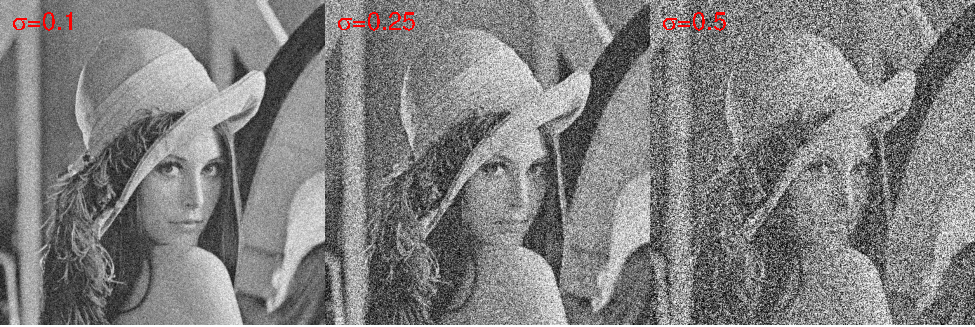
\includegraphics{project2_files/figure-latex/Nadaraya-Watson-estimator Lena-1.pdf}

\begin{verbatim}
## Gaussian kernel
\end{verbatim}

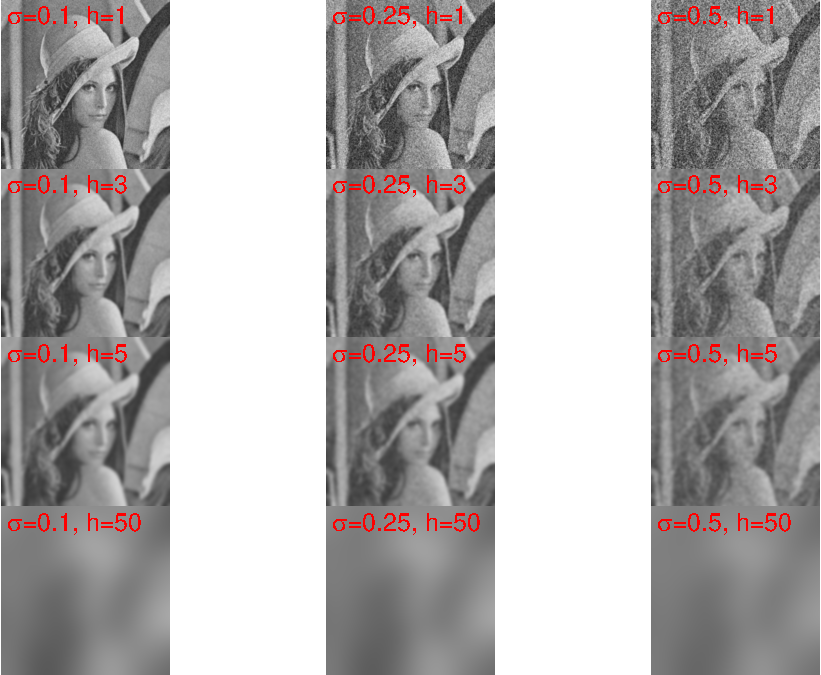
\includegraphics{project2_files/figure-latex/Nadaraya-Watson-estimator Lena-2.pdf}

\begin{verbatim}
## Rectangular kernel
\end{verbatim}

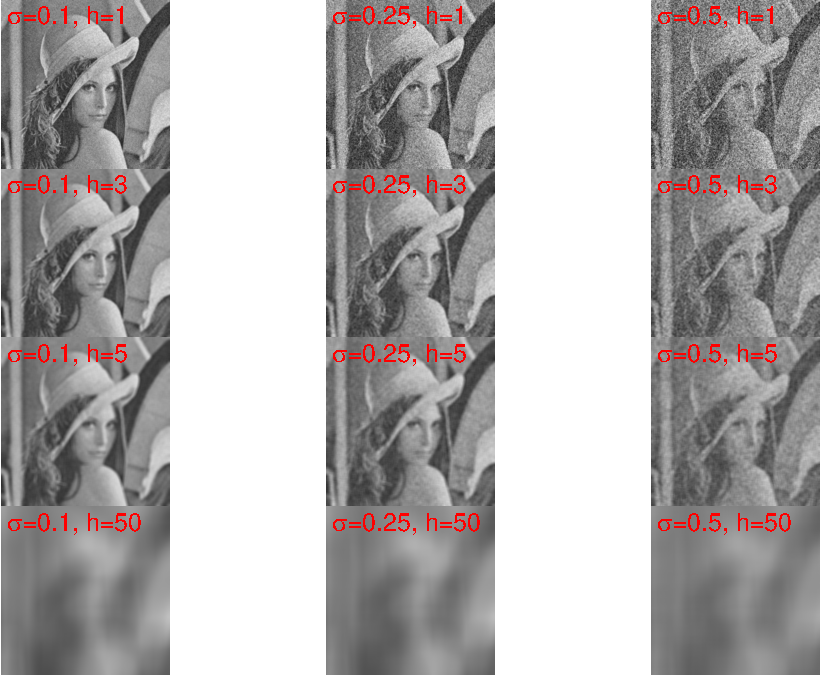
\includegraphics{project2_files/figure-latex/Nadaraya-Watson-estimator Lena-3.pdf}

Wir können sehen, dass natürlicherweise mit größerem Rauschniveau
\(\sigma\) das Bildentrauschen schwieriger fällt. Mit größerer Bandweite
\(h\) wird auch die Umgebung um den zu entrauschenden Pixel der für die
Schätzung gewichtigen Pixel größer, d.h.~die Schätzung ist das
gewichtete Mittel von Pixeln einer größeren Umgebung. In der Folge
verwischt das Bild stärker bzw.~wird weicher. Kanten verschmieren und
Kontraste zwischen den Farbflächen werden reduziert. Vergleichen wir die
Ergebnisse der beiden unterschiedlichen Kerne, so können wir sehen, dass
der Gaußkern „radial`` mittelt, wohingegen der Rechteckskern den Pixel
umschließende Quadrate zur Mittelung heranzieht. Tatsächlich steuert für
den Rechteckskern die Bandweite \(h\) genau die Größe des zur Mittelung
herngezogenen Quadrates. Wählt man \(h=1\), so werden nur alle dem zu
entrauschenden Pixel angrenzenden Pixel (sowie der Pixel selbst) zur
Mittelung benutzt. Somit erhalten wir für einen Pixel (der nicht am Rand
liegt) ein \(3\times3\) Quadrat über welches gemittelt wird. Allgemein
wird also für Pixel (die hinreichend weit vom Rand entfernt liegen) ein
\((2h+1) \times (2h+1)\) zur Mittelung herangezogen. Dieser Effekt wird
für die sehr große Bandweite \(h=50\) verdeutlicht. Hier ist beim
Entrauschen mit Rechtseckskern ein „Schachbrettmuster`` zu erkennen.

Wiederholen wir die Analyse für ein weiteres Bild \texttt{porsche.jpg}:

\begin{Shaded}
\begin{Highlighting}[]
\NormalTok{sigma <-}\StringTok{ }\KeywordTok{c}\NormalTok{(}\FloatTok{0.1}\NormalTok{, }\FloatTok{0.25}\NormalTok{, }\FloatTok{0.5}\NormalTok{)}
\NormalTok{h <-}\StringTok{ }\KeywordTok{c}\NormalTok{(}\DecValTok{1}\NormalTok{, }\DecValTok{3}\NormalTok{, }\DecValTok{5}\NormalTok{, }\DecValTok{50}\NormalTok{)}

\CommentTok{# Porsche}
\NormalTok{imgPorsche <-}\StringTok{ }\KeywordTok{readImage}\NormalTok{(}\StringTok{"porsche.jpeg"}\NormalTok{)}
\KeywordTok{fnEvalNWGaussianNoise}\NormalTok{(imgPorsche, sigma, h)}
\end{Highlighting}
\end{Shaded}

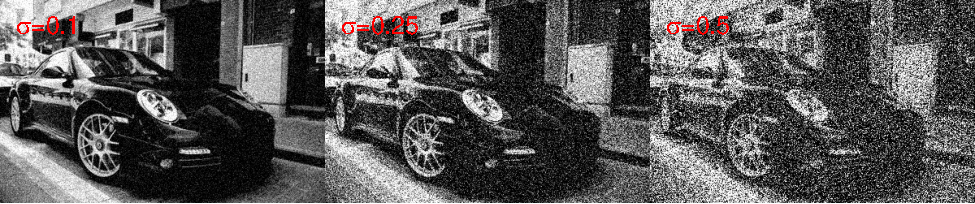
\includegraphics{project2_files/figure-latex/Nadaraya-Watson-estimator Porsche-1.pdf}

\begin{verbatim}
## Gaussian kernel
\end{verbatim}

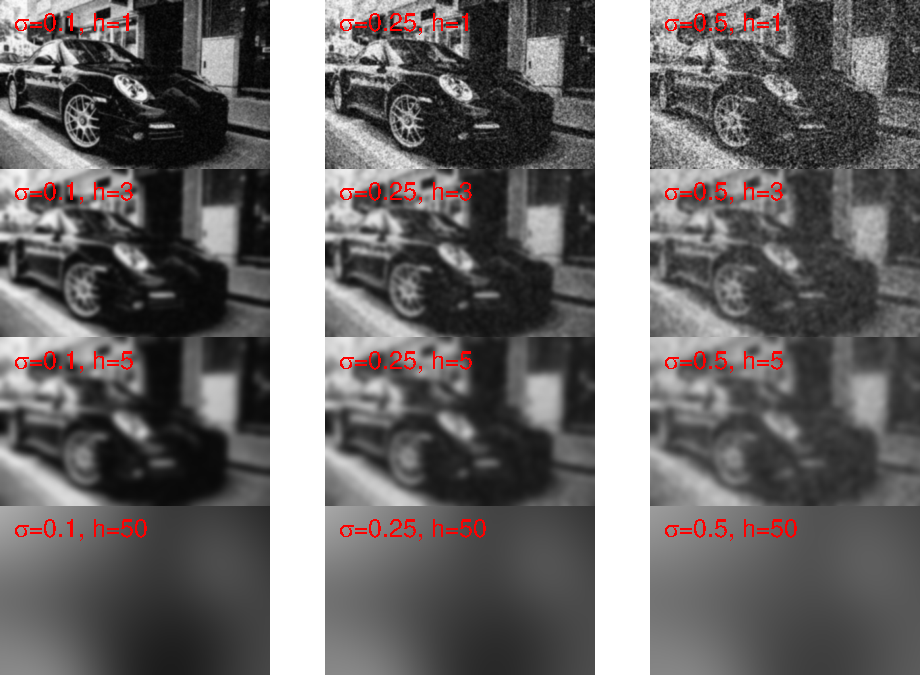
\includegraphics{project2_files/figure-latex/Nadaraya-Watson-estimator Porsche-2.pdf}

\begin{verbatim}
## Rectangular kernel
\end{verbatim}

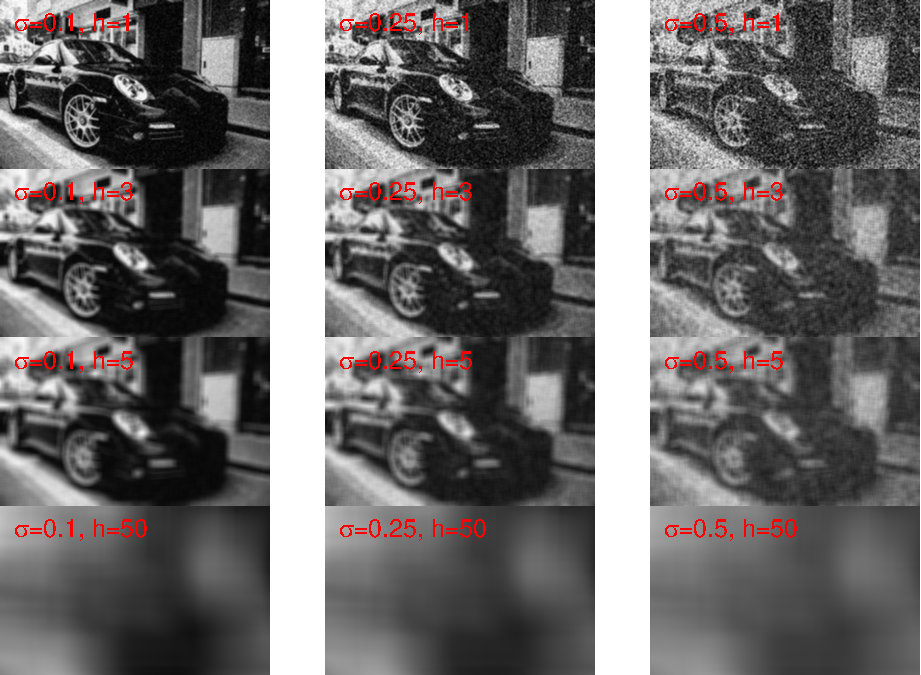
\includegraphics{project2_files/figure-latex/Nadaraya-Watson-estimator Porsche-3.pdf}

Beim Bildentrauschen von \texttt{porsche.jpg} sind dieselben Effekte wie
zuvor für verschiedene Bandweiten und Rauschniveaus sowie die beiden
unterschiedlichen Kerne zu beobachten.

Abschließend wollen wir den Nadaraya-Watson-Schätzer auf Robustheit
untersuchen und dazu die Bilder mit nicht normalverteiltem Rauschen
belegen. Stattdessen wählen wir \(t\)-verteiltes Rauschen, wodurch
häufiger Ausreißer generiert werden:

\begin{Shaded}
\begin{Highlighting}[]
\NormalTok{fnEvalNWCauchyNoise <-}\StringTok{ }\NormalTok{function(img, vdf, vh) \{}
  \CommentTok{# This function is a wrapper to compare the denoising results of images with }
  \CommentTok{# different levels of t-distributed noise for the Nadaraya-Watson-estimator }
  \CommentTok{# with weights defined by the Gaussian kernel and rectangular kernel}
  \CommentTok{# respectively for different bandwidths h.}
  \CommentTok{# }
  \CommentTok{# Args:}
  \CommentTok{#   img:  Image}
  \CommentTok{#   vdf:  Vector of degrees of freedom used to add noise}
  \CommentTok{#   vh:   Vector of bandwidths used in weights of the}
  \CommentTok{#         Nadaraya-Watson-estimator}
  \CommentTok{#   }
  \CommentTok{# Returns:}
  \CommentTok{#   -}
  
  \CommentTok{# Define helper function for label implementation}
  \NormalTok{fnLabel <-}\StringTok{ }\NormalTok{function(label) \{}
    \KeywordTok{text}\NormalTok{(}\DataTypeTok{x =} \DecValTok{20}\NormalTok{, }\DataTypeTok{y =} \DecValTok{20}\NormalTok{, }\DataTypeTok{adj =} \KeywordTok{c}\NormalTok{(}\DecValTok{0}\NormalTok{,}\DecValTok{1}\NormalTok{), }\DataTypeTok{col =} \StringTok{"red"}\NormalTok{, }\DataTypeTok{cex =} \FloatTok{1.5}\NormalTok{, }\DataTypeTok{label =} \NormalTok{label)}
  \NormalTok{\}}
  
  \CommentTok{# Set size of frame}
  \KeywordTok{par}\NormalTok{(}\DataTypeTok{mfrow =} \KeywordTok{c}\NormalTok{(}\DecValTok{1}\NormalTok{, }\KeywordTok{length}\NormalTok{(vdf)))}
  
  \CommentTok{# Initalize noise image list}
  \NormalTok{imagesNoise <-}\StringTok{ }\KeywordTok{list}\NormalTok{()}
  
  \NormalTok{for (i in }\DecValTok{1}\NormalTok{:}\KeywordTok{length}\NormalTok{(vdf)) \{}
    \CommentTok{# Add noise to image and plot}
    \NormalTok{imgNoise <-}\StringTok{ }\KeywordTok{fnAddNoise}\NormalTok{(img, rt, }\DataTypeTok{df =} \NormalTok{vdf[i])}
    \NormalTok{imagesNoise[i] <-}\StringTok{ }\KeywordTok{list}\NormalTok{(imgNoise)}
    \KeywordTok{display}\NormalTok{(imgNoise, }\DataTypeTok{method =} \StringTok{"raster"}\NormalTok{)}
    \KeywordTok{fnLabel}\NormalTok{(}\KeywordTok{substitute}\NormalTok{(}\KeywordTok{paste}\NormalTok{(}\StringTok{"df="}\NormalTok{, df), }\KeywordTok{list}\NormalTok{(}\DataTypeTok{df=}\NormalTok{vdf[i])))}
  \NormalTok{\}}
  
  \CommentTok{# Set size of frame for plots below}
  \KeywordTok{par}\NormalTok{(}\DataTypeTok{mfrow =} \KeywordTok{c}\NormalTok{(}\KeywordTok{length}\NormalTok{(vh), }\KeywordTok{length}\NormalTok{(vdf)))}
  
  \KeywordTok{cat}\NormalTok{(}\StringTok{'Gaussian kernel'}\NormalTok{)}
  \NormalTok{for (h in vh) \{}
    \CommentTok{# NW-Denoising with Gaussian kernel}
    \NormalTok{for (i in }\DecValTok{1}\NormalTok{:}\KeywordTok{length}\NormalTok{(vdf)) \{}
      \KeywordTok{display}\NormalTok{(}\KeywordTok{fnNadarayaWatson}\NormalTok{(imagesNoise[[i]], fnGaussianKernel, h),}
              \DataTypeTok{method =} \StringTok{"raster"}\NormalTok{)}
      \KeywordTok{fnLabel}\NormalTok{(}\KeywordTok{substitute}\NormalTok{(}\KeywordTok{paste}\NormalTok{(}\StringTok{"df="}\NormalTok{, df, }\StringTok{", h="}\NormalTok{, h),}
                         \KeywordTok{list}\NormalTok{(}\DataTypeTok{df=}\NormalTok{vdf[i], }\DataTypeTok{h=}\NormalTok{h)))}
    \NormalTok{\}}
  \NormalTok{\}}
  
  \KeywordTok{cat}\NormalTok{(}\StringTok{'Rectangular kernel'}\NormalTok{)}
  \NormalTok{for (h in vh) \{ }
    \CommentTok{# NW-Denoising with rectangular kernel}
    \NormalTok{for (i in }\DecValTok{1}\NormalTok{:}\KeywordTok{length}\NormalTok{(vdf)) \{}
      \KeywordTok{display}\NormalTok{(}\KeywordTok{fnNadarayaWatson}\NormalTok{(imagesNoise[[i]], fnRectangularKernel, h), }
              \DataTypeTok{method =} \StringTok{"raster"}\NormalTok{)}
      \KeywordTok{fnLabel}\NormalTok{(}\KeywordTok{substitute}\NormalTok{(}\KeywordTok{paste}\NormalTok{(}\StringTok{"df="}\NormalTok{, df, }\StringTok{", h="}\NormalTok{, h),}
                         \KeywordTok{list}\NormalTok{(}\DataTypeTok{df=}\NormalTok{vdf[i], }\DataTypeTok{h=}\NormalTok{h)))}
    \NormalTok{\}}
  \NormalTok{\}}
\NormalTok{\}}
\end{Highlighting}
\end{Shaded}

Betrachten wir erneut die Ergebnisse für \texttt{lena.png}:

\begin{Shaded}
\begin{Highlighting}[]
\NormalTok{df <-}\StringTok{ }\KeywordTok{c}\NormalTok{(}\DecValTok{100}\NormalTok{, }\DecValTok{50}\NormalTok{, }\DecValTok{1}\NormalTok{)}
\NormalTok{h <-}\StringTok{ }\KeywordTok{c}\NormalTok{(}\DecValTok{1}\NormalTok{, }\DecValTok{3}\NormalTok{, }\DecValTok{5}\NormalTok{, }\DecValTok{50}\NormalTok{)}

\CommentTok{# Lena}
\KeywordTok{fnEvalNWCauchyNoise}\NormalTok{(imgLenaGray, df, h)}
\end{Highlighting}
\end{Shaded}

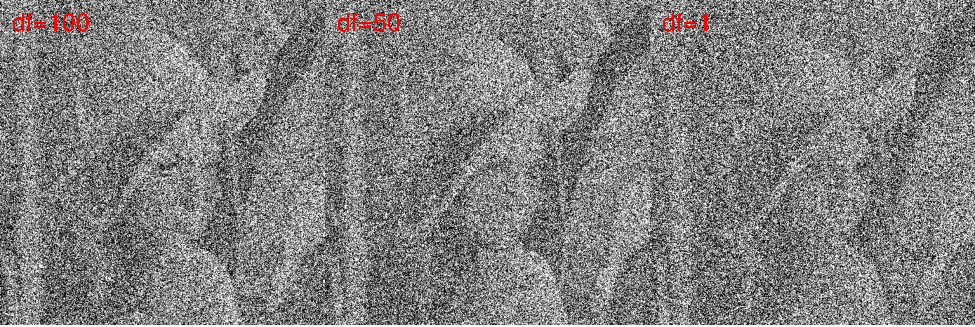
\includegraphics{project2_files/figure-latex/Nadaraya-Watson-estimator non-Gaussian Noise Lena-1.pdf}

\begin{verbatim}
## Gaussian kernel
\end{verbatim}

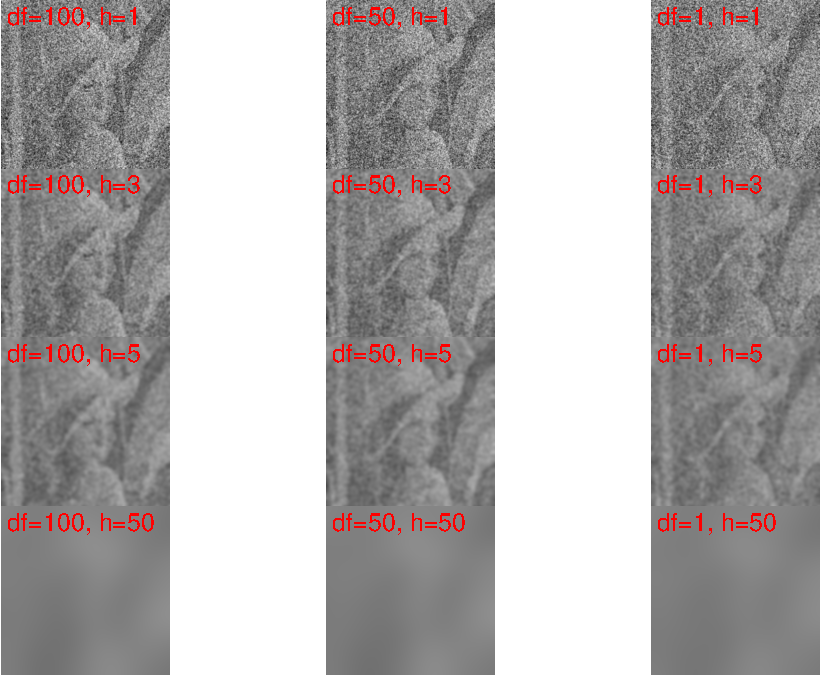
\includegraphics{project2_files/figure-latex/Nadaraya-Watson-estimator non-Gaussian Noise Lena-2.pdf}

\begin{verbatim}
## Rectangular kernel
\end{verbatim}

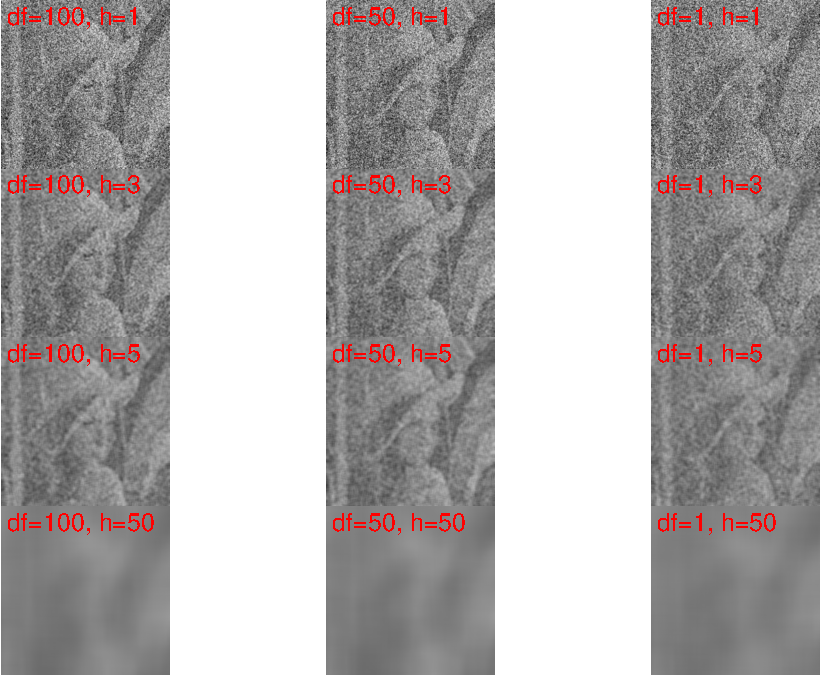
\includegraphics{project2_files/figure-latex/Nadaraya-Watson-estimator non-Gaussian Noise Lena-3.pdf}

Um einen robusteren Schätzer zur erhalten könnten wir, wie in der
parametrischen Regression, anstelle der kleinsten quadratischen Abstände
die kleinsten absoluten Abstände betrachten, d.h.~folgendes Problem
betrachten:

\[
\argmin_{y \in [0,1]} \left( \sum_{k=1}^m \sum_{l=1}^p | Y_{kl} - y | \, w_{kl}(i,j) \right).
\]

Die Lösung des Problems ist dann der gewichtete Median, d.h.~für das
geordnetes sample \(Y^{(1)}_{k_1l_1}, \ldots, Y^{(mp)}_{k_{mp},l_{mp}}\)
mit Gewichten \(w_{k_1l_1}(i,j), \ldots, w_{k_{mp},l_{mp}}(i,j)\)
erfüllt der gewichtete Median \(Y^{(M)}_{k_{M},l_{M}}\) \[
\sum_{t=1}^{M-1} w_{k_tl_t}(i,j) < \frac{1}{2} \quad \text{und} \quad \sum_{t=M+1}^{mp} w_{k_tl_t}(i,j) \leq \frac{1}{2}.
\]

\subsection{Weitere Methoden zur
Bildentrauschung}\label{weitere-methoden-zur-bildentrauschung}

\subsubsection{Rangordnungsfilter}\label{rangordnungsfilter}

Bei Rangordnungsfilter wird eine bestimmte Anzahl von Grauwerten in
einer Umgebung eines Pixels betrachtet. Die so erfassten Grauwerte
werden dem Rang nach in einer Liste sortiert, also nach Größe des
Grauwertes. Der aktuell betrachtete Pixel wird durch einen Grauwert aus
der Liste ersetzt. Dabei kann für die Wahl der Position ein beliebiges
Verfahren eingesetzt werden, z.B. Minimumfilter (minimaler Wert aus der
Liste), Maximumfilter (maximaler Wert aus der Liste), Medianfilter (der
Grauwert in der Mitte der Liste), etc.

Rangordnungsfilter eignen sich für Bilder mit Ausreißern, also z.B.
Kratzer oder einzelne deutlich abweichende Pixel.

\subsubsection{Frequenzraumfilter}\label{frequenzraumfilter}

Ein Bild kann sowohl im Ortsraum, als auch im Freuqenzraum beschrieben
werden. Zur Transformation aus dem Ortsraum in den Frequenzraum wird
eine diskrete Fouriertransformation durchgeführt. Anschließend können
verschiedene Filter verwendet werden, z.B. Hochpass- oder
Tiefpassfilter. Zufälliges Rauschen kann als hochfrequent angenommen
werden, weshalb sich hier ein Tiefpassfilter eignen würde (die niedrigen
Frequenzen bleiben unverändert). Dabei kann der Filter ``hart''
abschneiden oder einen Übergangsbereich definieren. Nach der Filterung
werden die Daten wieder in den Ortsraum zurück transformiert.

Anwednungsfälle für den Frequenzraumfilter ergeben sich je nach
Fragestellung. Für verschiedene Fälle eignen sich entsprechende Filter
im Frequenzraum.


\end{document}
